\documentclass[useAMS,usenatbib]{mn2e}
\bibliographystyle{mn2e}
\pdfoutput=1
\pdfminorversion=5

%\usepackage{widetext}
\usepackage{graphicx}
\usepackage{dcolumn}
\usepackage{bm}
\usepackage{amssymb,amsmath,bm,dsfont}
\usepackage{color}
\usepackage[dvipsnames]{xcolor}
\usepackage[colorlinks,linkcolor=red,citecolor=blue,urlcolor=blue ]{hyperref}
\usepackage{multirow}
\usepackage[utf8]{inputenc}
\usepackage{balance}
\usepackage{enumitem}
\usepackage{lipsum}
\newcommand{\nv}{\hat{\bf n}}
\newcommand{\kalo}{Karhunen-Lo\`{e}ve~}
\newcommand{\cfh}{CFHTLenS~}
\newcommand{\jcap}{JCAP}
\newcommand{\mnras}{MNRAS}
\newcommand{\aap}{A\&A}
\newcommand{\aaps}{A\&AS}
\newcommand{\apjs}{ApJS}
\newcommand{\apj}{ApJ}
\newcommand{\apjl}{ApJL}
\newcommand{\prd}{Phys.~Rev.~D}
\newcommand{\prl}{Phys.~Rev.~Lett.}
\newcommand{\aj}{Astron. Journal}
\newcommand{\pasp}{Publications of the ASP}
\newcommand{\nar}{New Astronomy Review}
\newcommand{\procspie}{Proceedings of the SPIE}
\newcommand{\physrep}{Physics Reports}

\newcommand{\todo}[1]{{\bf TODO: #1}}
%\newcommand{\todo}[1]{$\,$}

\newcommand{\pcl}[3]{\hat C_{#1}^{#2 #3}}
\newcommand{\avg}[1]{\langle #1 \rangle}
\newcommand{\fsky}{f_{\mbox{\rm sky}}}
\newcommand{\clth}{C_\ell^{th}}
\newcommand{\clf}{C_\ell^{fore}}
\newcommand{\cl}{C_\ell}
\newcommand{\summ}[1]{\sum_{\bf #1}\Delta #1^2}
\newcommand{\Ylm}[3]{{\sf E}^{#1}_{\bf #2}({\bf #3})}
\newcommand{\red}[1]{{\color{red} #1}}

\title[Disconnected pseudo-$C_\ell$ covariances for projected datasets]{Disconnected pseudo-$C_\ell$ covariances for projected datasets}
\author[C. Garc\'{i}a-Garc\'{i}a et al.]{Carlos Garc\'{i}a-Garc\'{i}a$^{1,\,2}$\thanks{carlosgarcia@iff.csic.es}, David Alonso$^2$\thanks{david.alonso@physics.ox.ac.uk}, Emilio Bellini$^2$\thanks{emilio.bellini@physics.ox.ac.uk}\\
$^{1}$ Instituto de Física Fundamental, Consejo Superior de Investigaciones
Científicas, c/. Serrano 123, E–28006, Madrid, Spain\\
$^{2}$Oxford Astrophysics, Department of Physics, Keble Road, Oxford, OX1 3RH, UK
}

\begin{document}
  \date{\today}
  \pagerange{1--18} \pubyear{2019}
  \maketitle

\begin{abstract}
\end{abstract}

\begin{keywords}
  cosmology: large-scale structure of the Universe -- methods: data analysis
\end{keywords}

\section{Introduction}
    
\section{Analytical Gaussian covariances}

  \subsection{Preliminaries}
    We will deal with spin-0 and spin-2 fields defined on a 2-dimensional space. We will use a generic notation that can then be applied to both curved and flat skies. Given a field ${\bf a}({\bf x})$, with 1 (spin-0) or 2 components (spin-2), and defined on the coordinates ${\bf x}$, we define its generalized Fourier coefficients as
    \begin{equation}
      {\bf a}_{\bf k}=\summ{x}\,\Ylm{\dag}{k}{x}\,{\bf a}({\bf x}),
    \end{equation}
    where the operator $\summ{x}$ denotes a integral or sum of all coordinates ${\bf x}$, and $\Ylm{\dag}{k}{x}$ are a set of orthogonal functions. We will also assume that the $\Ylm{\dag}{k}{x}$ are a \emph{complete} set of basis functions, in which case:
    \begin{align}
      &\summ{x}\,\Ylm{\dag}{k}{x}\Ylm{}{l}{x}=\mathds{1}\Delta^x({\bf k},{\bf l}),\\
      &\summ{k}\,\Ylm{}{k}{x}\Ylm{\dag}{k}{y}=\mathds{1}\Delta^k({\bf x},{\bf y}),
    \end{align}
    where $\summ{k}$ denotes an integral over all possible generalised Fourier coefficients ${\bf k}$, and $\Delta^x$ and $\Delta^k$ are generalized delta functions:
    \begin{align}
      &\summ{k}\,f({\bf k})\Delta^x({\bf k},{\bf l})\equiv f({\bf l}),\\
      &\summ{x}\,f({\bf x})\Delta^k({\bf x},{\bf y})\equiv f({\bf y}).
    \end{align}
    
    Finally, we will assume that all fields are Gaussian stochastic fields that are additionally statistically isotropic. As a consequence of this, different generalised Fourier modes are uncorrelated:
    \begin{equation}
      \langle {\bf a}_{\bf k}{\bf b}^\dag_{\bf l}\rangle\equiv {\sf C}^{ab}_k\,F\,\Delta^x({\bf k},{\bf l}),
    \end{equation}
    where $F$ is a volume factor (see below) and ${\sf C}^{ab}_k$ is the power spectrum.
    
    All the functions and operators above can be specialised to fields defined on the sphere or the 2D plane (flat sky) as follows:
    
  
  \subsection{The pseudo-$C_\ell$ method}
  
  \subsection{Covariance matrices}

This section presents the analytical approximations used here to estimate the pseudo-$C_\ell$ Gaussian covariance matrix.

This section presents the analytical calculation of the pseudo-$C_\ell$ covariance. The treatment and approximations used are similar to those presented in \todo{cite} for spin-0 quantities, in \todo{cite} for particular spin-0 and spin-2 correlations and in \todo{cite} for the 3D density field. We reproduce the formalism here in order to provide a complete set of formulas applicable to any cross-correlation in both curved and flat skies.



\begin{itemize}
\item Naive Covariance
  \begin{equation}
    C^{abcd} = \frac{\pcl{l}ad \pcl{l}bc + \pcl{l}ac \pcl{l}bd}{f_{sky} (2l +
      1) \Delta l} \delta_{ll'}
    \label{eq:naive}
  \end{equation}
\item Approximation 1
\item Approximation 2
\end{itemize}

\section{Results}
For both flat and curved sky we should discuss:
\begin{itemize}
\item Simulations (sims, methods)
\item Approximation 1 - spin 0
\item Approximation 1 - spin 2
\item Approximation 2
\item Naive
\end{itemize}

For both flat and curved plots:
\begin{itemize}
\item Cov Naive
\item Cov approx 1
\item Cov approx 2
\item Cov approx 2 + deprojection
\end{itemize}

Plots:
\begin{itemize}
\item Plot $\chi^2$
\item KS($\chi^2$)
\item Eigenvalues
\end{itemize}

In this section we will show that our approximation is good and reliable; i.e.
that can be used to obtain the cosmological parameters within the same error
as using the covariance matrix from simulations. 

\subsection{Simulations}

Simulations were drawn from Gaussian fields that followed a fiducial power
spectrum. The fiducial cosmology (\red{For the 2-bin case}) is given by
$\Omega_{cdm} = 0.27$, $\Omega_b = 0.045$, $h = 0.67$, $A_s = 2.1 10^{-9}$ and
$n_s = 0.9$, where each term correspond, respectively, to the amount of cold
dark matter and baryons today, the reduced Hubble constant, the primordial
curvature fluctuation amplitude and the spectral index. The redshift bins are
shown in Fig.~\ref{fig:pz} and the theoretical $\cl$ are in
Fig.~\ref{fig:cl-2bins}. Since all parts of sky will not be equally observed, a
realist mask (see Fig.~\ref{fig:mask}) was applied.  The results shown here
were obtained using the same mas for each redshift bin, as it is expected to
be that way in real observations. We checked, however, that using different
masks yielded same results. 

\begin{figure}
  \centering
  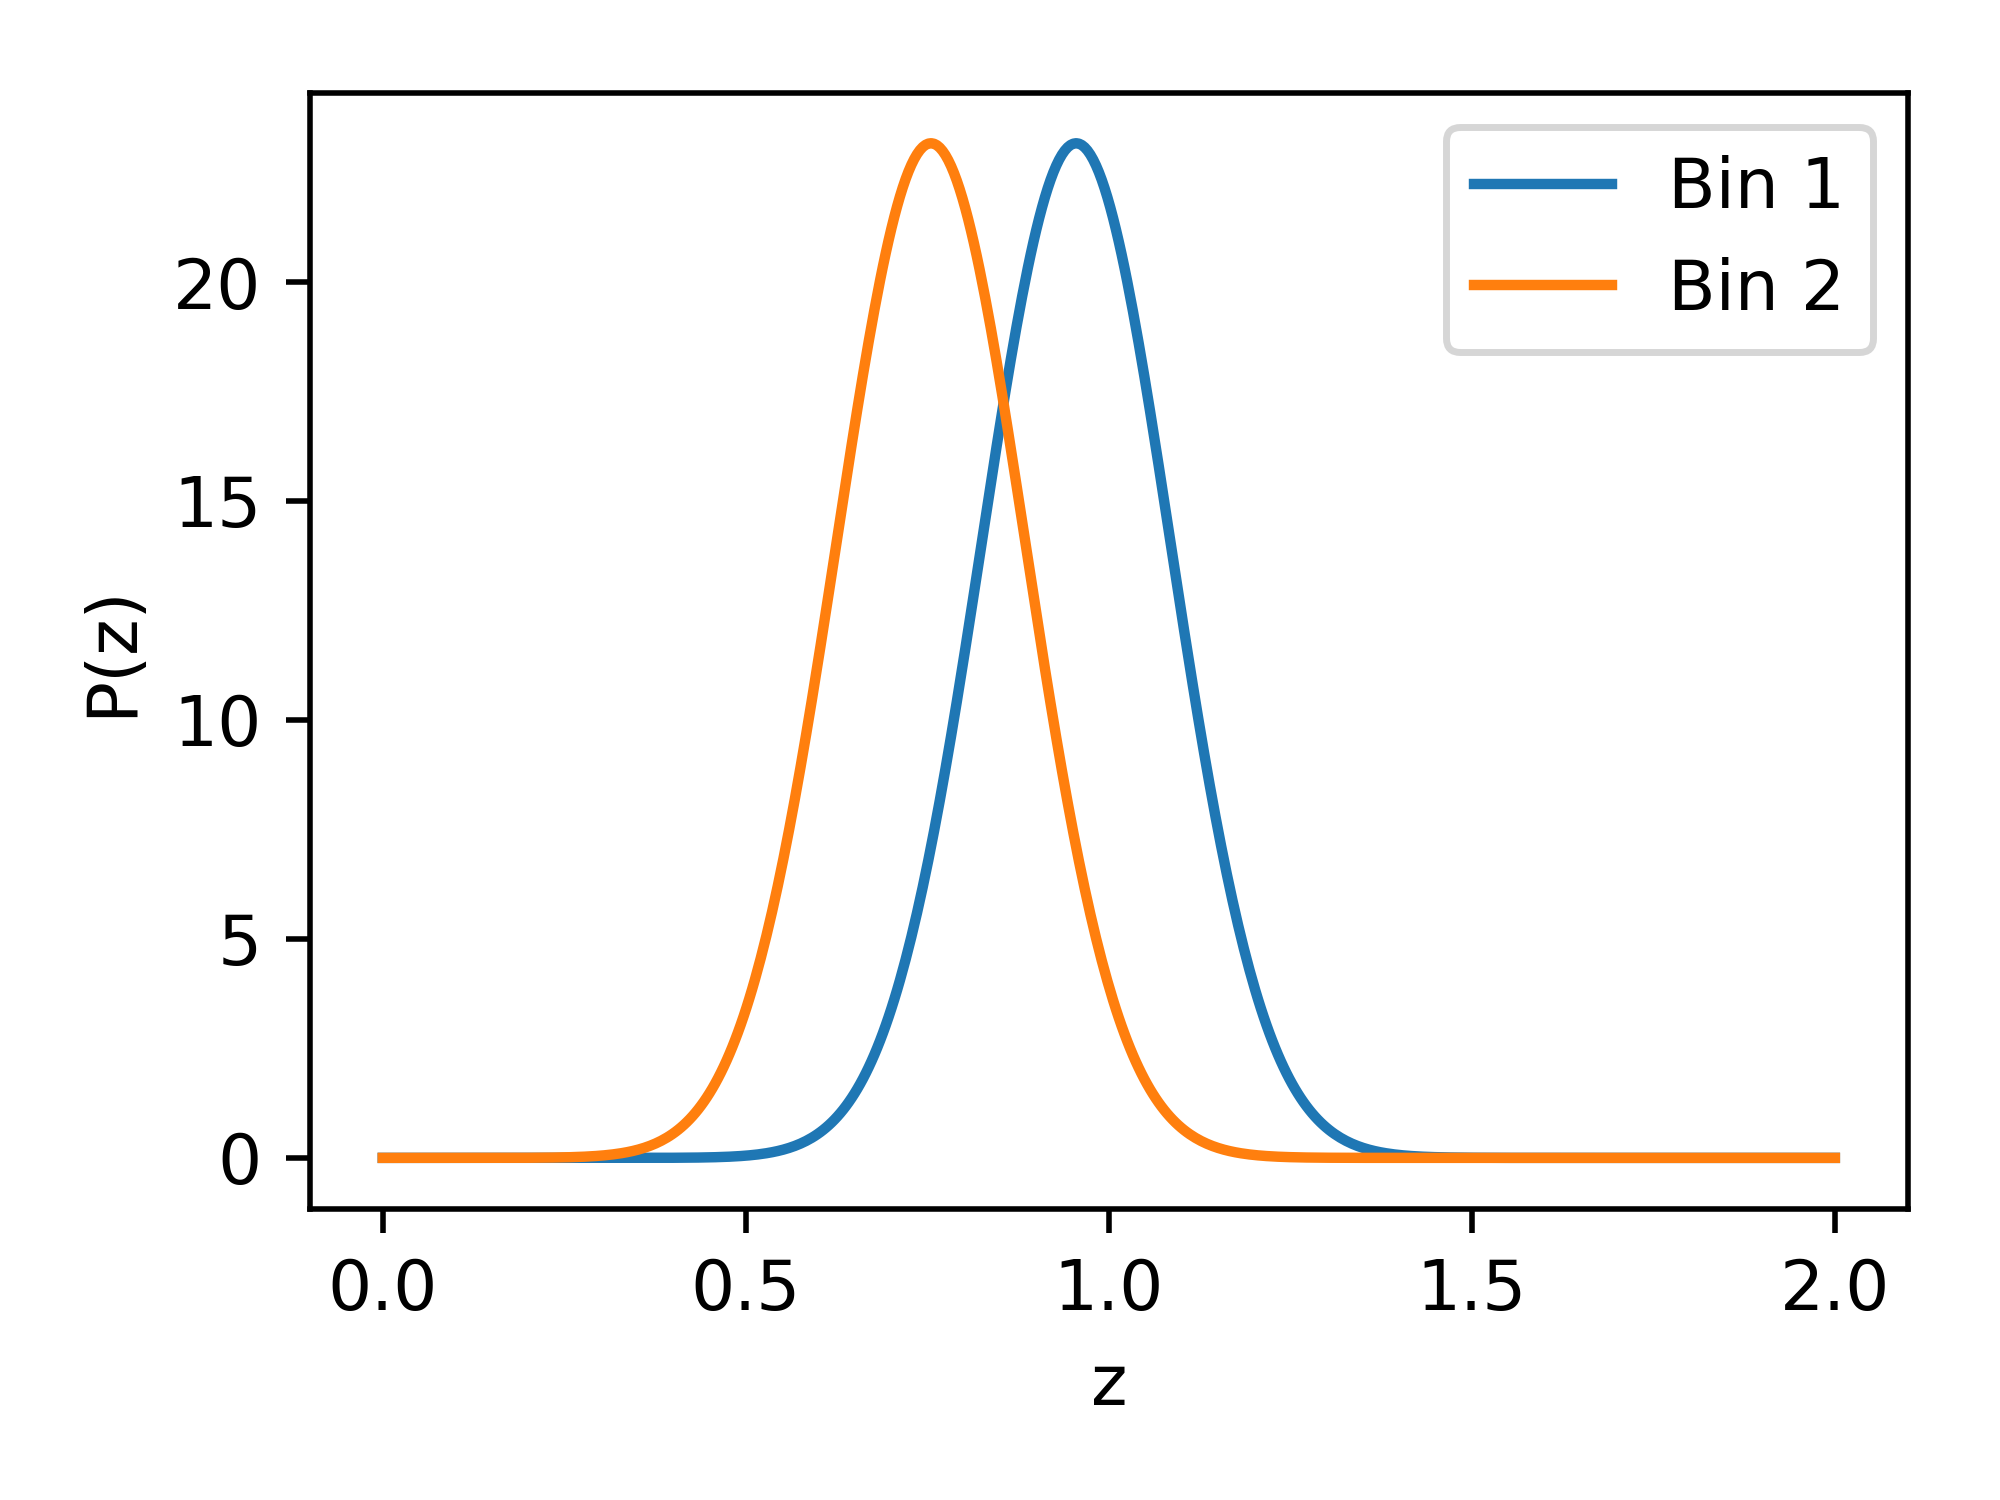
\includegraphics[width=\columnwidth]{./figures/pz.png}
  \caption{Galaxy distribution redshift bins.}
  \label{fig:pz}
\end{figure}

\begin{figure*}
  \centering
  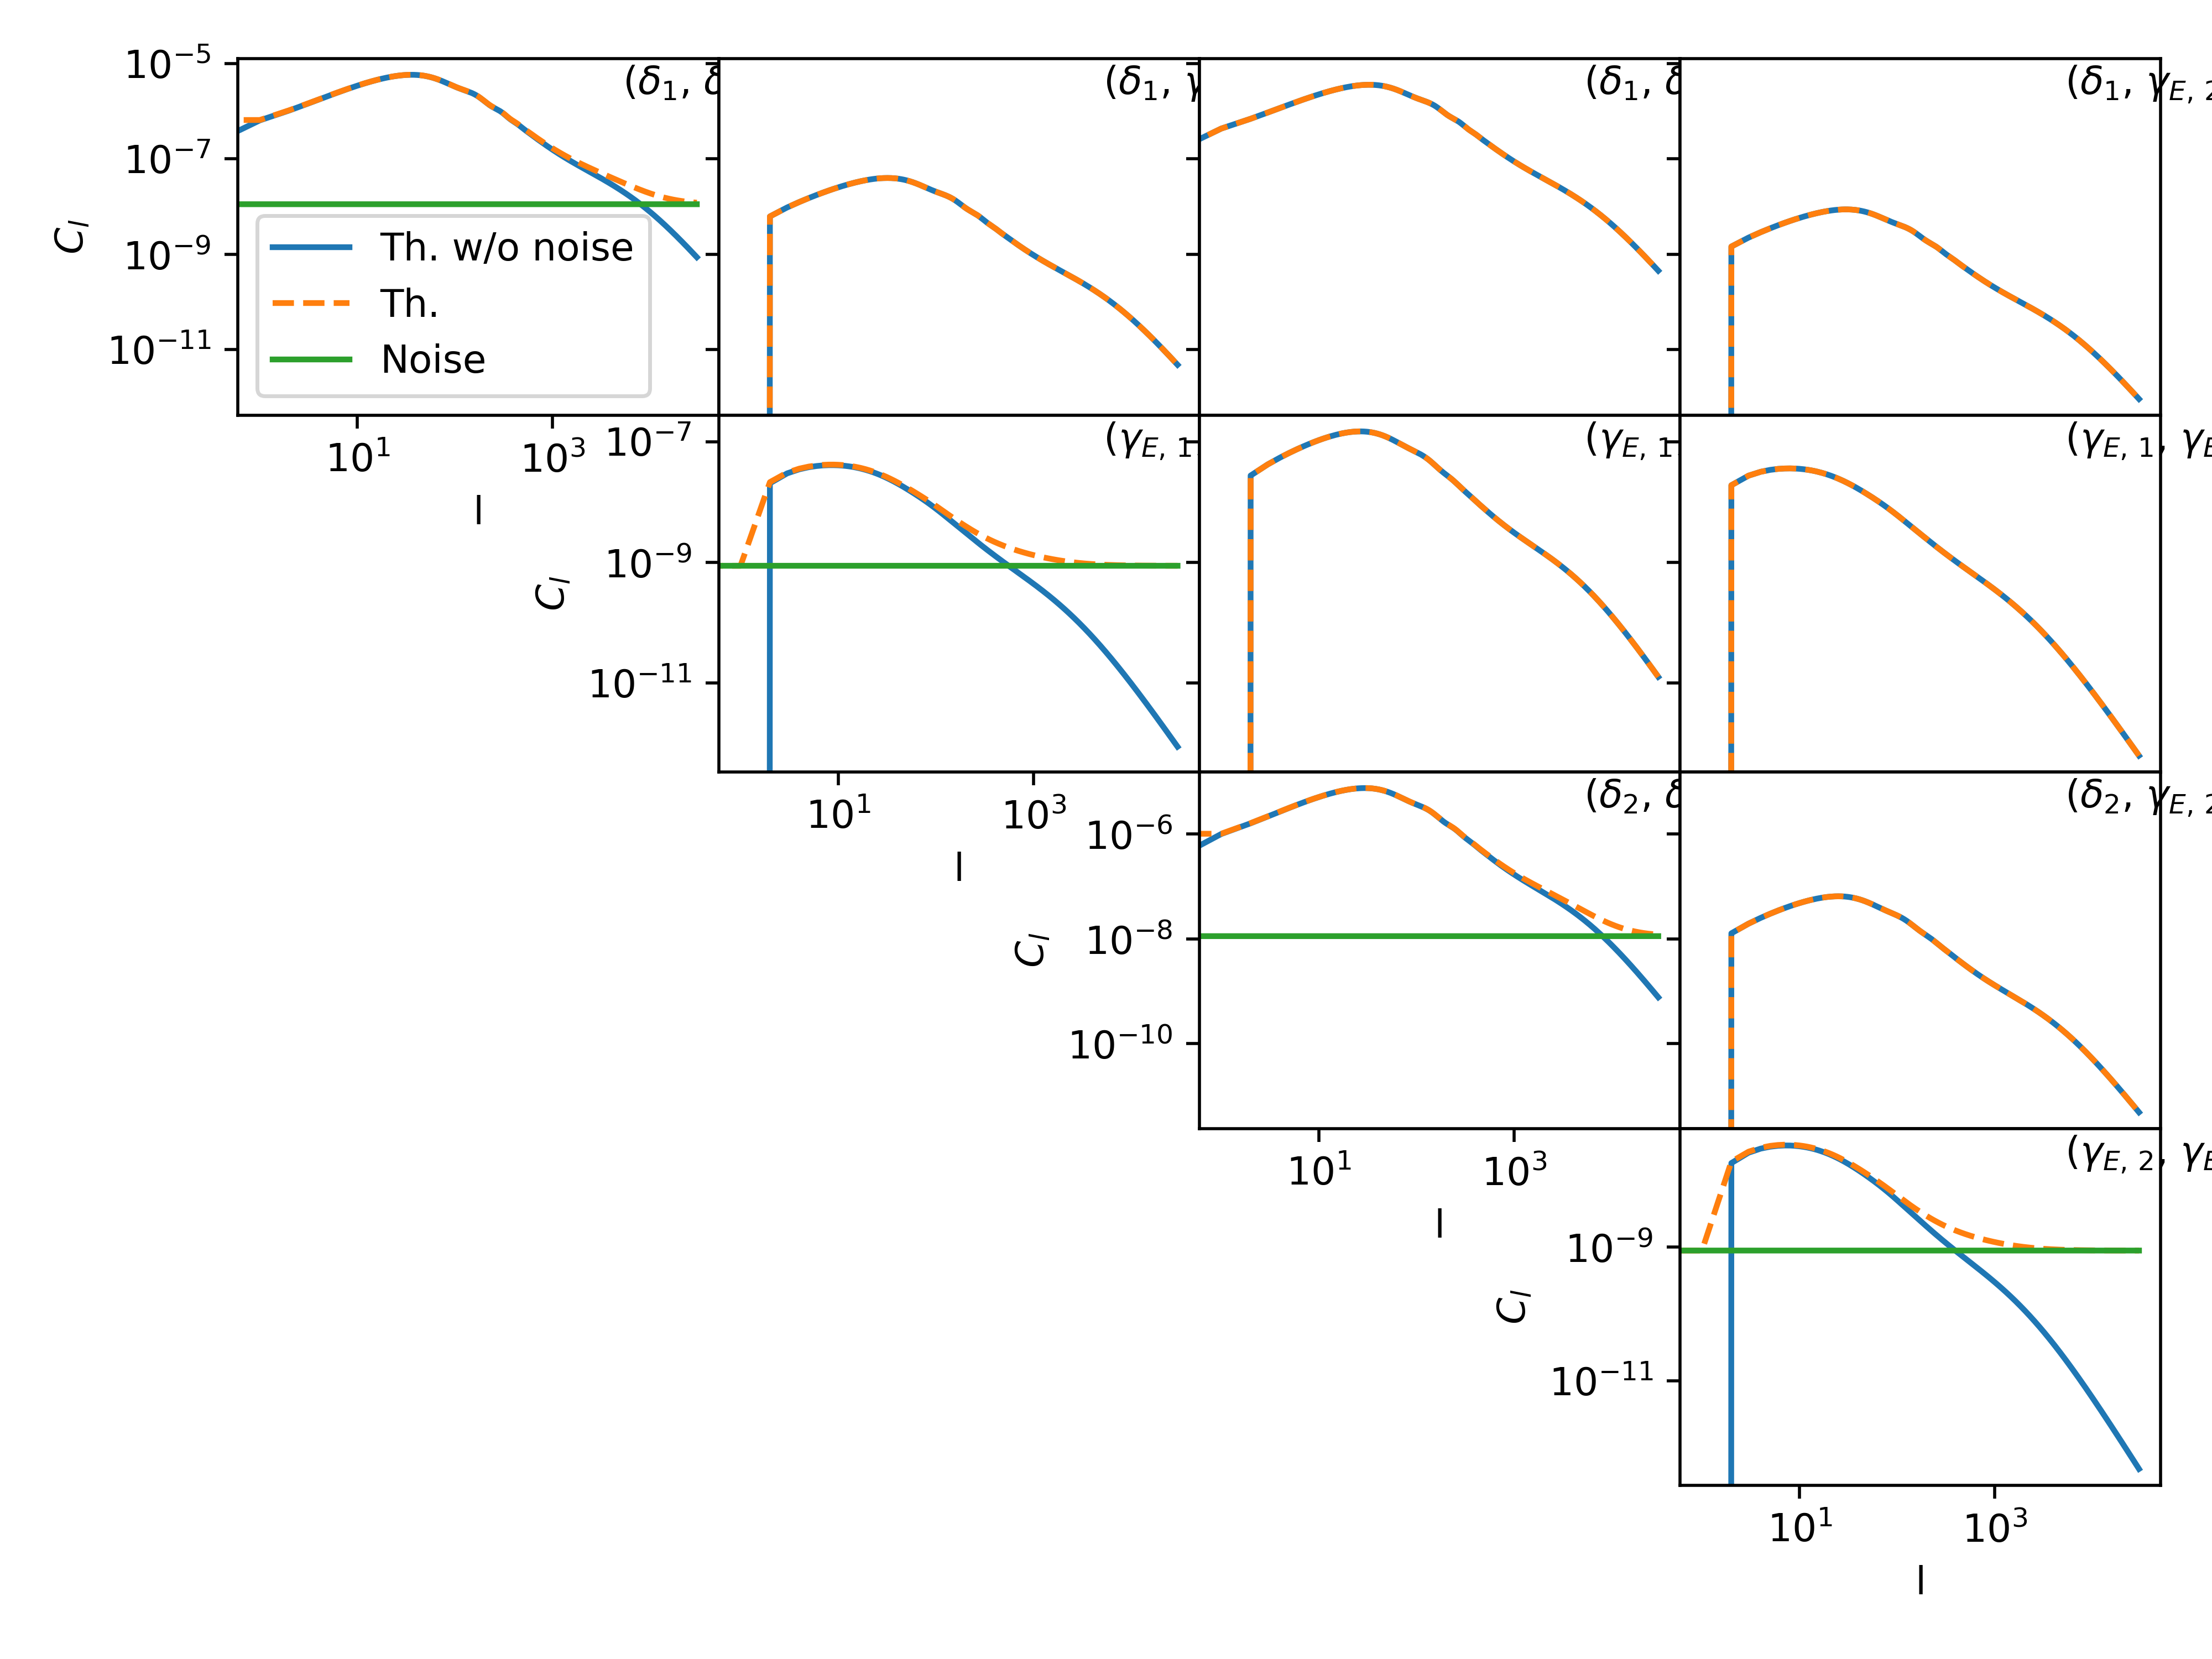
\includegraphics[width=\textwidth]{./figures/cls-sph-2b.png}
  \caption{Fiducial power spectra. We show only the $T$ and $E$ modes.}
  \label{fig:cl-2bins}
\end{figure*}

\begin{figure}
  \centering
  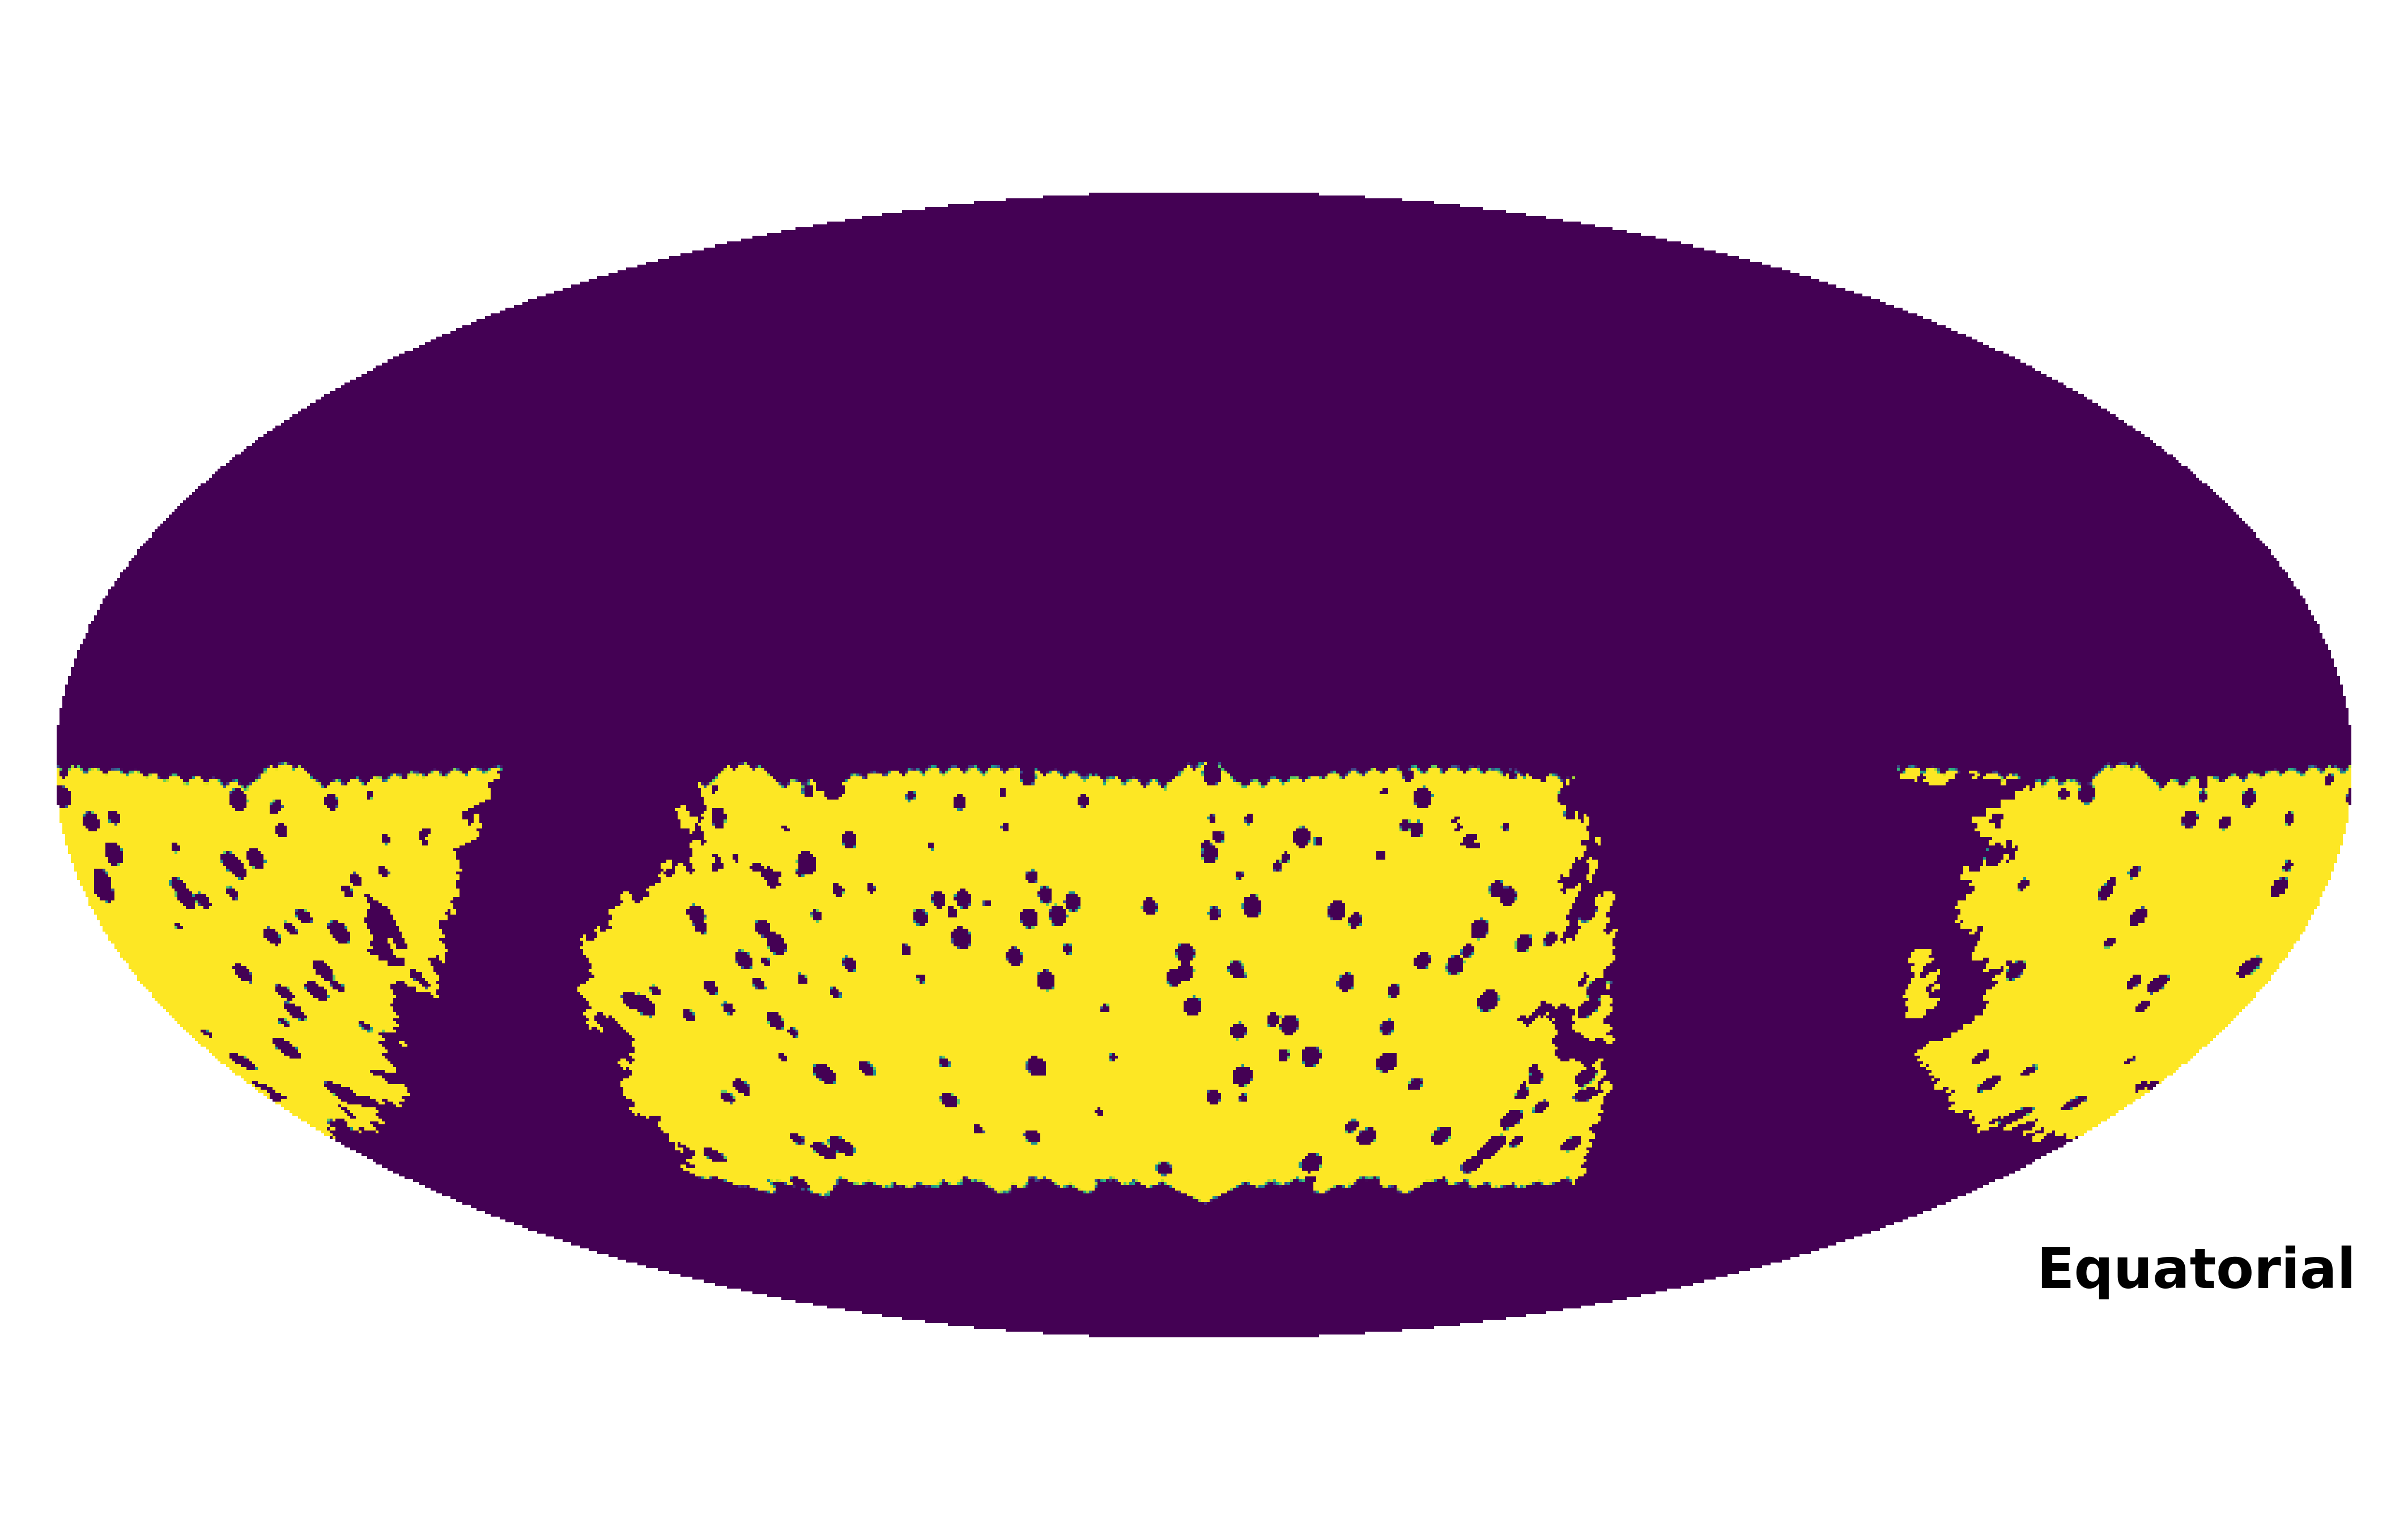
\includegraphics[width=\columnwidth]{./figures/mask-lss1.png}
  \caption{Example of sky mask used in our analysis}
  \label{fig:mask}
\end{figure}

The covariance matrices were obtained from 20000 simulations, for the band
powers determined by the fraction of sky observed and the maximum band power
we were able to recover the fiducial power spectra for; i.e. $\sim 2 \times
512$. This corresponds to $l_{\mbox{bpw}} = 1023$. To work with the sky
maps and masks we used
\textit{HEALPix}\footnote{\url{https://healpix.jpl.nasa.gov/}}, whereas 
\textit{NaMaster}\footnote{\url{https://github.com/LSSTDESC/NaMaster}}~\cite{2018arXiv180909603A}
was used for the computation of the pseudo-$\cl$ and the covariances. Our code
is publicly
available~\footnote{\url{https://github.com/damonge/PCLCovariance}}.

The same results are obtained even in the presence of foregrounds. In
particular, we tested the case with 100 foregrounds both at low scales and
large scales, adding a mock power spectra (e.g. Fig.~\ref{fig:fore}) computed as 
\begin{equation}
  \clf = A (l + 1)^{\beta}\,.
  \label{eq:fore}
\end{equation}
Here, $A$ was fixed so that the ratio of the foreground power spectra and the
theoretical one ($\clth$) was $\clf/\clth = 0.1$ at $l=400$ and $\beta$ was
randomly chosen from $U[-3, -1)$ for large scale effects and fixed to $\beta =
0$ for small scale ones. 

\begin{figure}
  \centering
  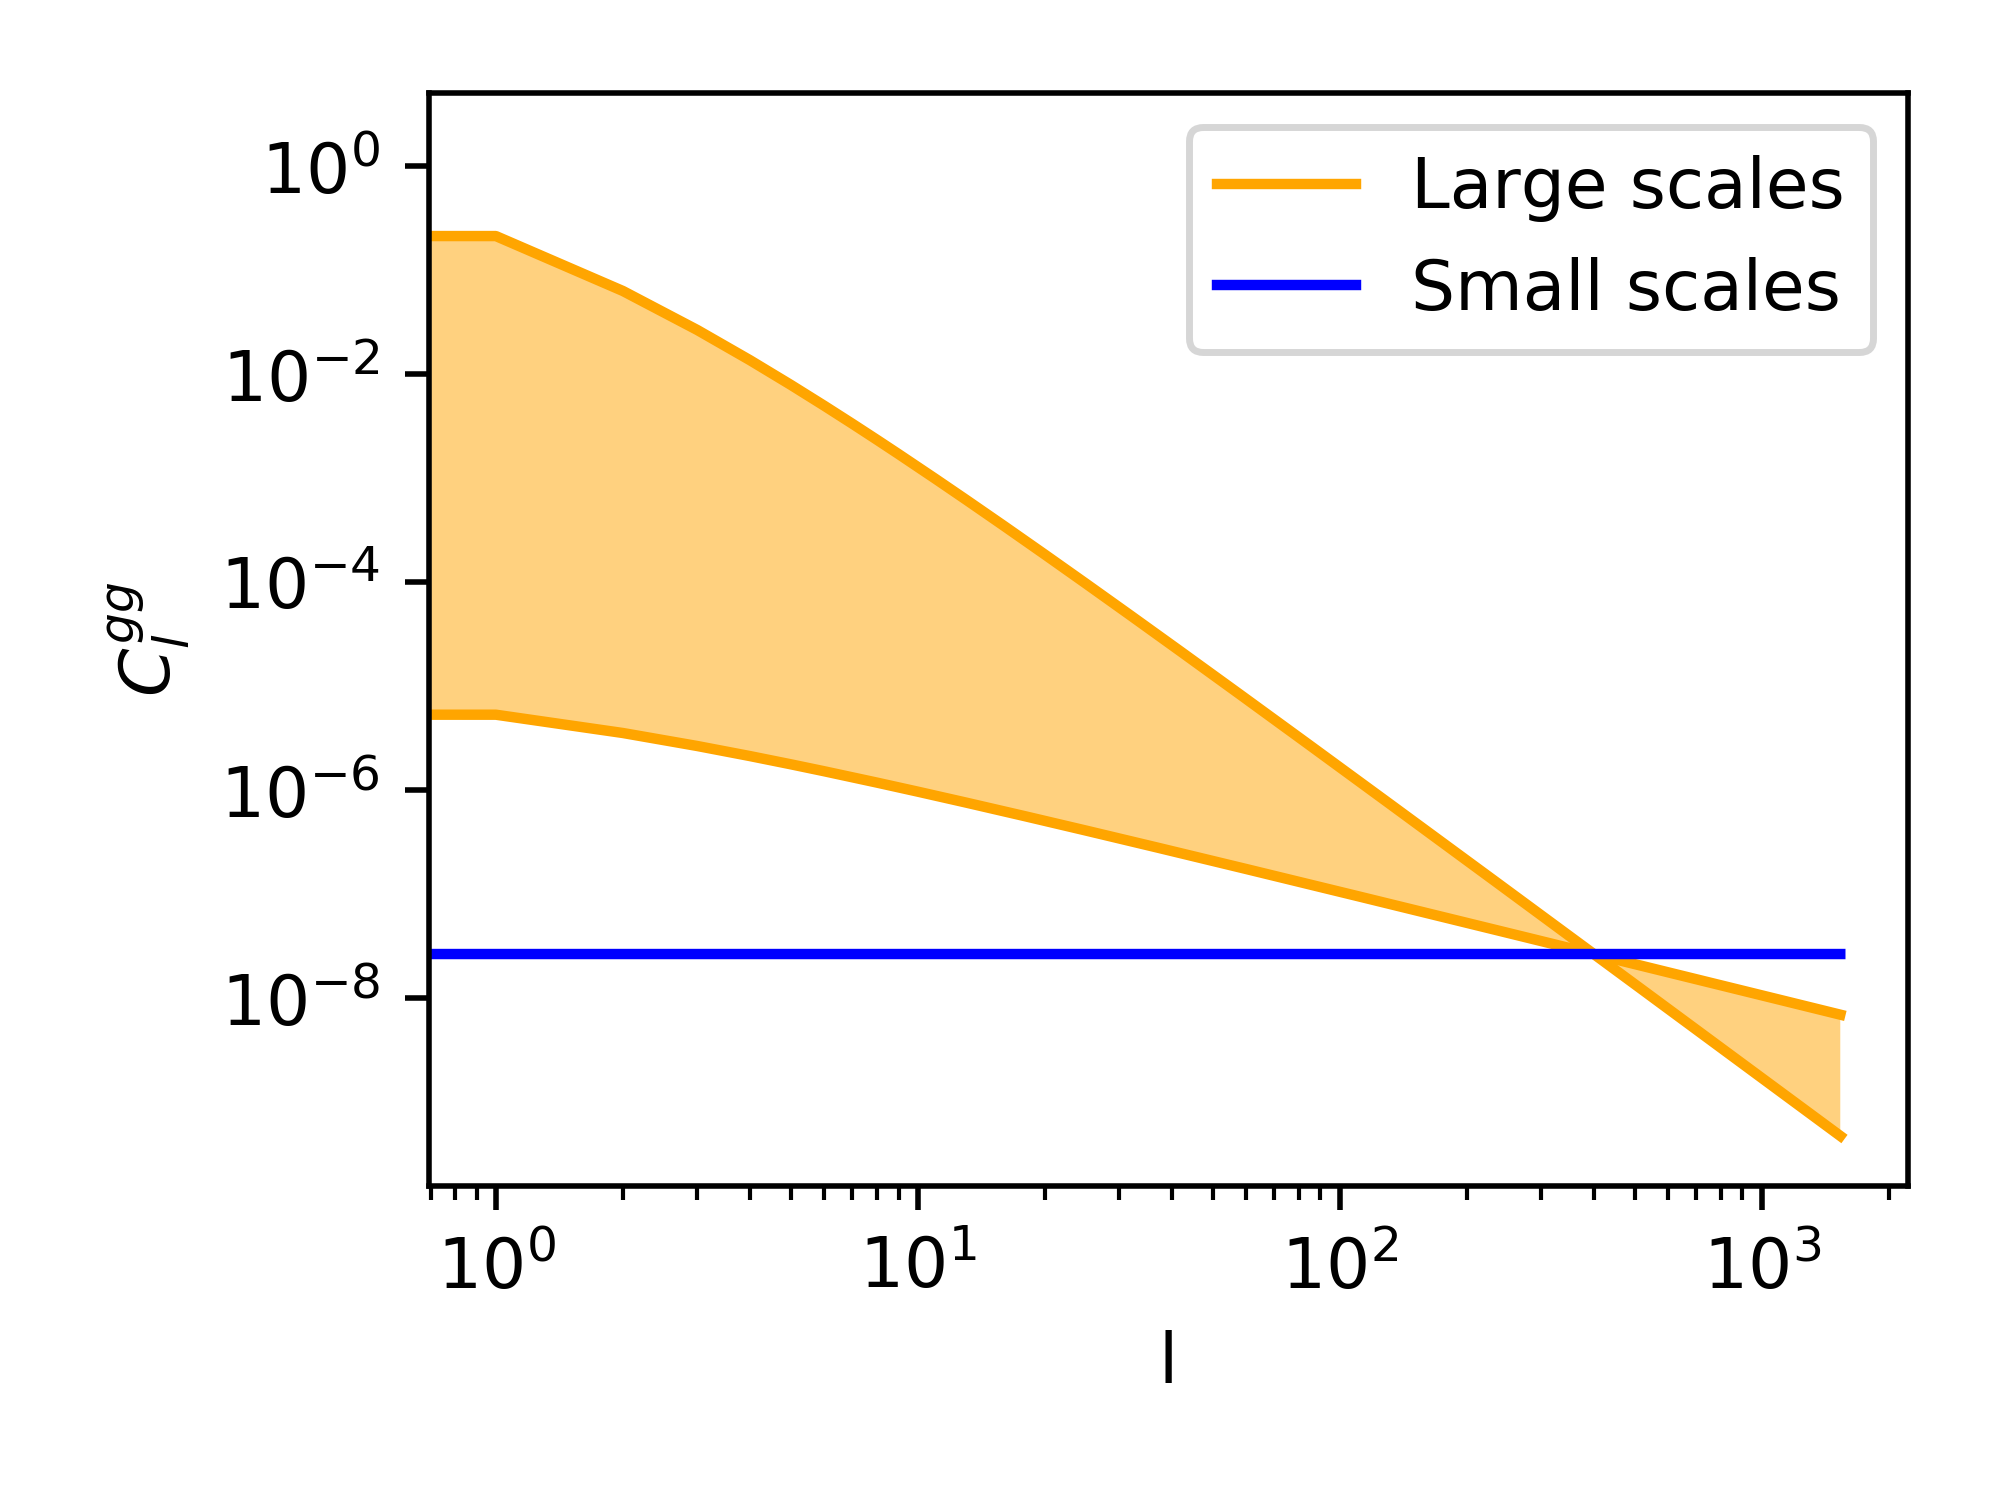
\includegraphics[width=\columnwidth]{./figures/foreground.png}
  \caption{$\cl$ foregrounds used in order to check the reliability of the
    analytical approximations in their presence. They did not affect. The
    limiting cases for the large-scale contaminants are given by $\beta=-1,\,
    -3$ in Eq.~\ref{eq:fore}}
  \label{fig:fore}
\end{figure}

\subsection{$\chi^2$ distribution and covariance matrices}
Apart from checking that we recover the same cosmological predictions from the
covariance matrices from both the analytical approximation and the
simulations, we studied the differences between them.

In this sense, one can see in Fig.~\ref{fig:TTTT_EEEE_chi2} that, we fully
recover the $\chi^2$ distribution (defining $\chi^2 = \cl - \langle \cl
\rangle C^{-1} \cl - \langle \cl \rangle$) for the TTTT case; whereas for the
worst case (i.e. EEEE) we are able to recover its shape, although sifted
toward lower values. This might be consequence of the fact that the inverse of
the covariance matrix is biased. It is interesting to note that even
the approximation of the mixing matrix as that of the case with spin 0, gives
good results. The eigenvalues of the covariance matrix
(Fig.~\ref{fig:TTTT_EEEE_eigv}) are also recovered within the 1\%, for all
scales in the TTTT case, and for the smaller scales in the EEEE case. Finally,
the analytical approximations are shown to describe the scale coupling (see
Fig.~\ref{fig:TTTT_rows} that comes from the fact we are masking some regions
of the sky. The larger relative deviation for the better approximations are
due to the fact that there is a division by $0$, while for the naive
approximation, which is defined diagonal (see Eq.~\ref{eq:naive}), the
relative deviation is exactly $-1$ for all values with $l \neq l'$.

\begin{figure*} %[htb]
  \centering
  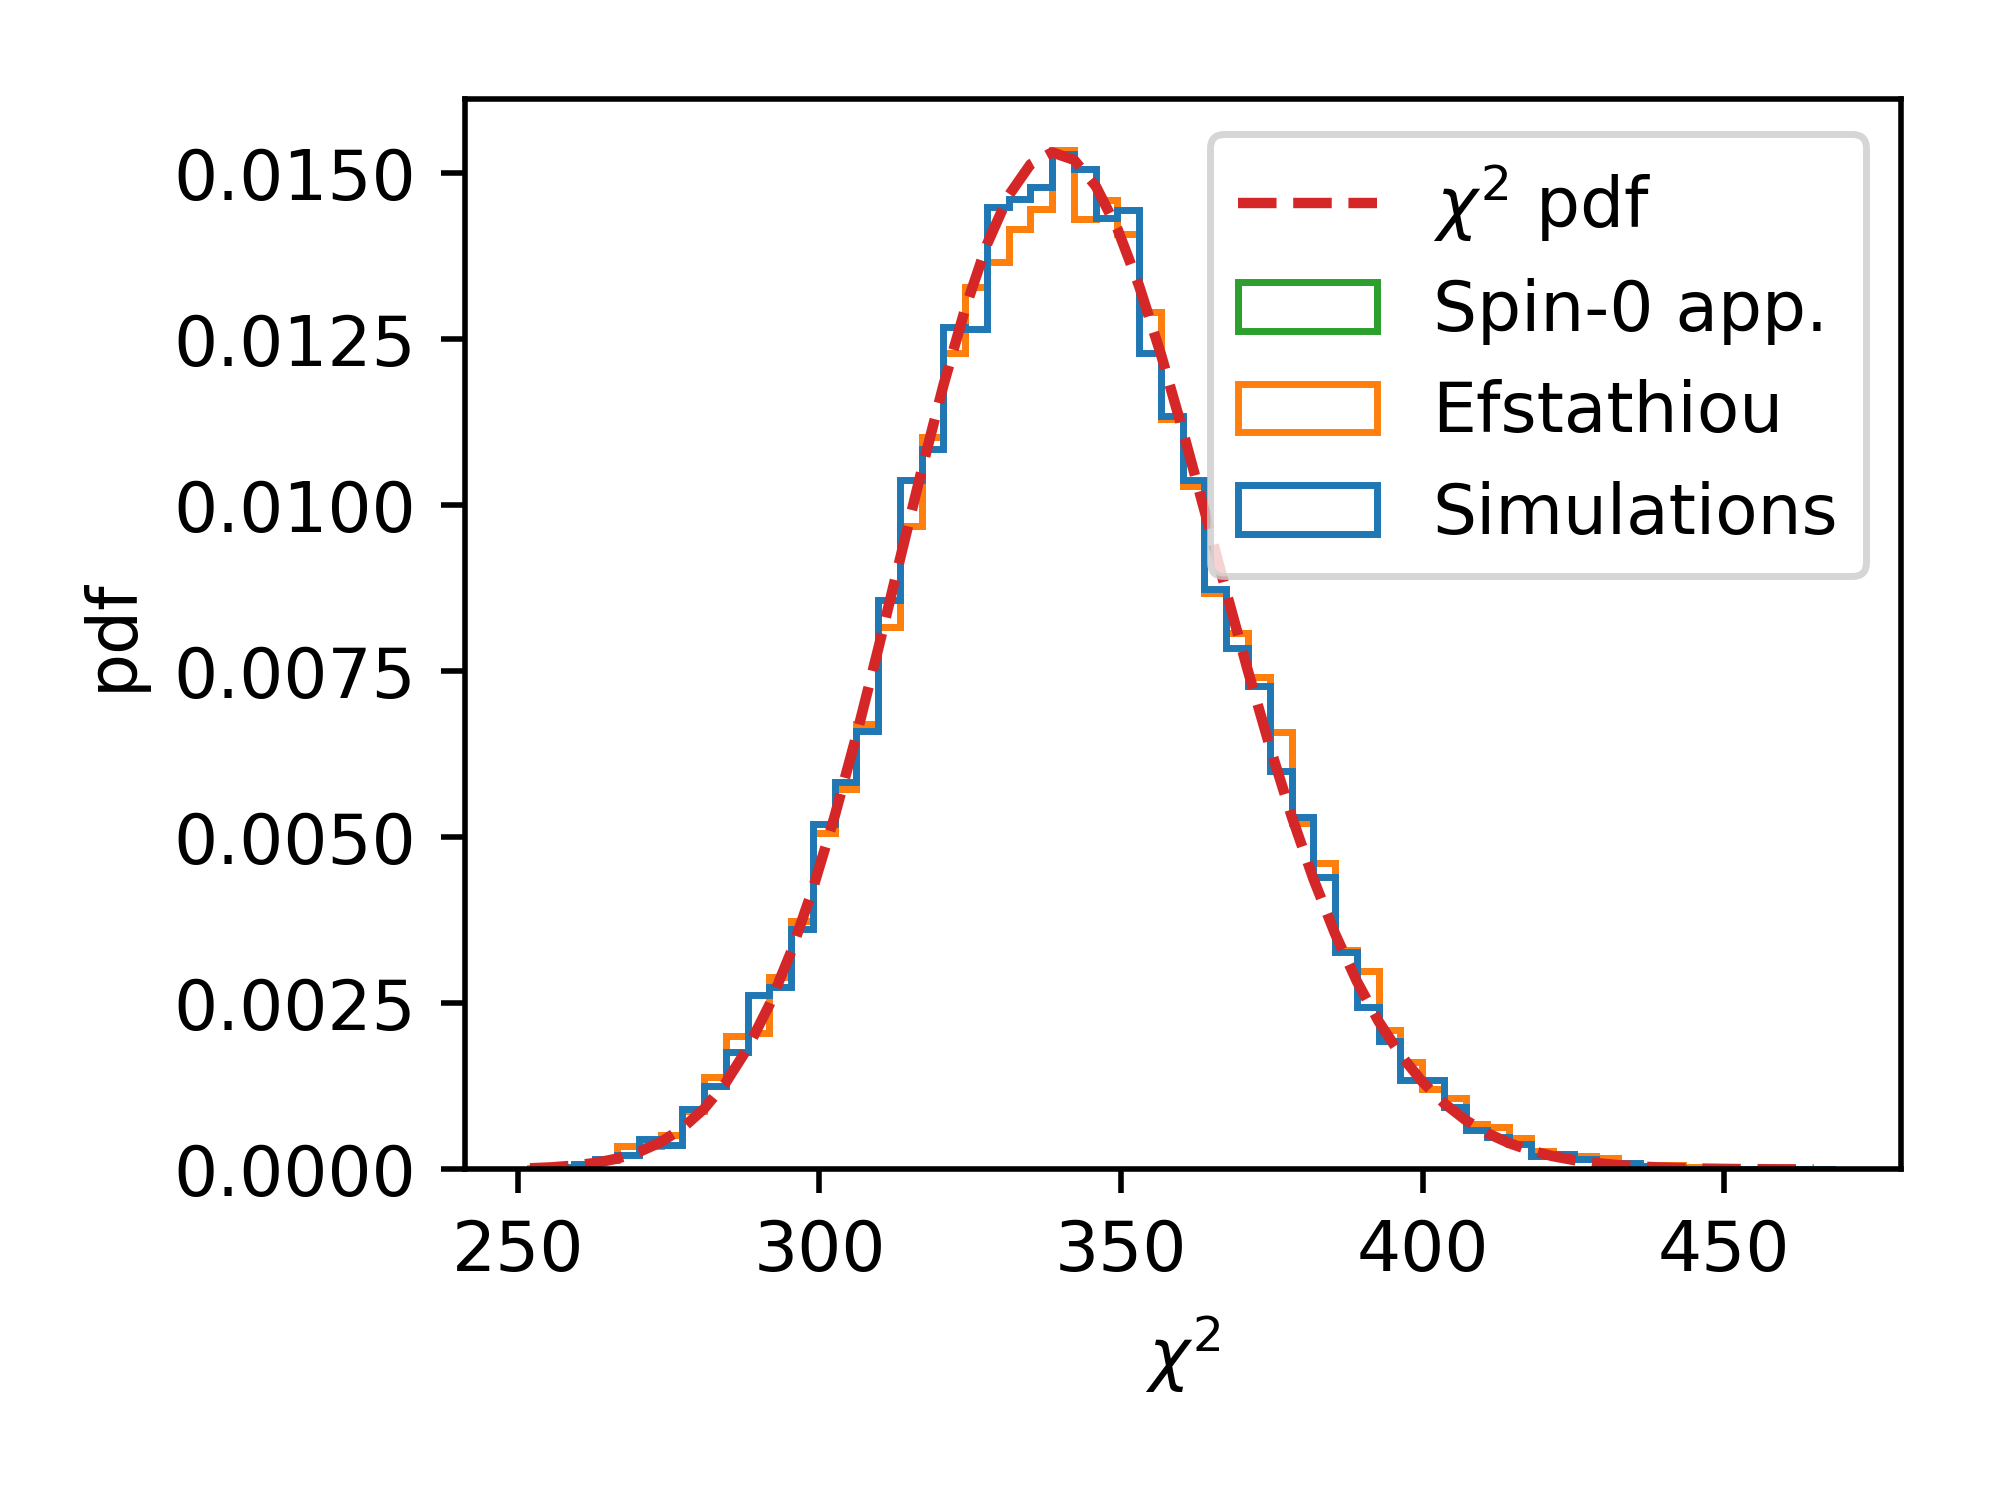
\includegraphics[width=\columnwidth]{./figures/run_sph_ALL_TTTT_chi2.png}~
  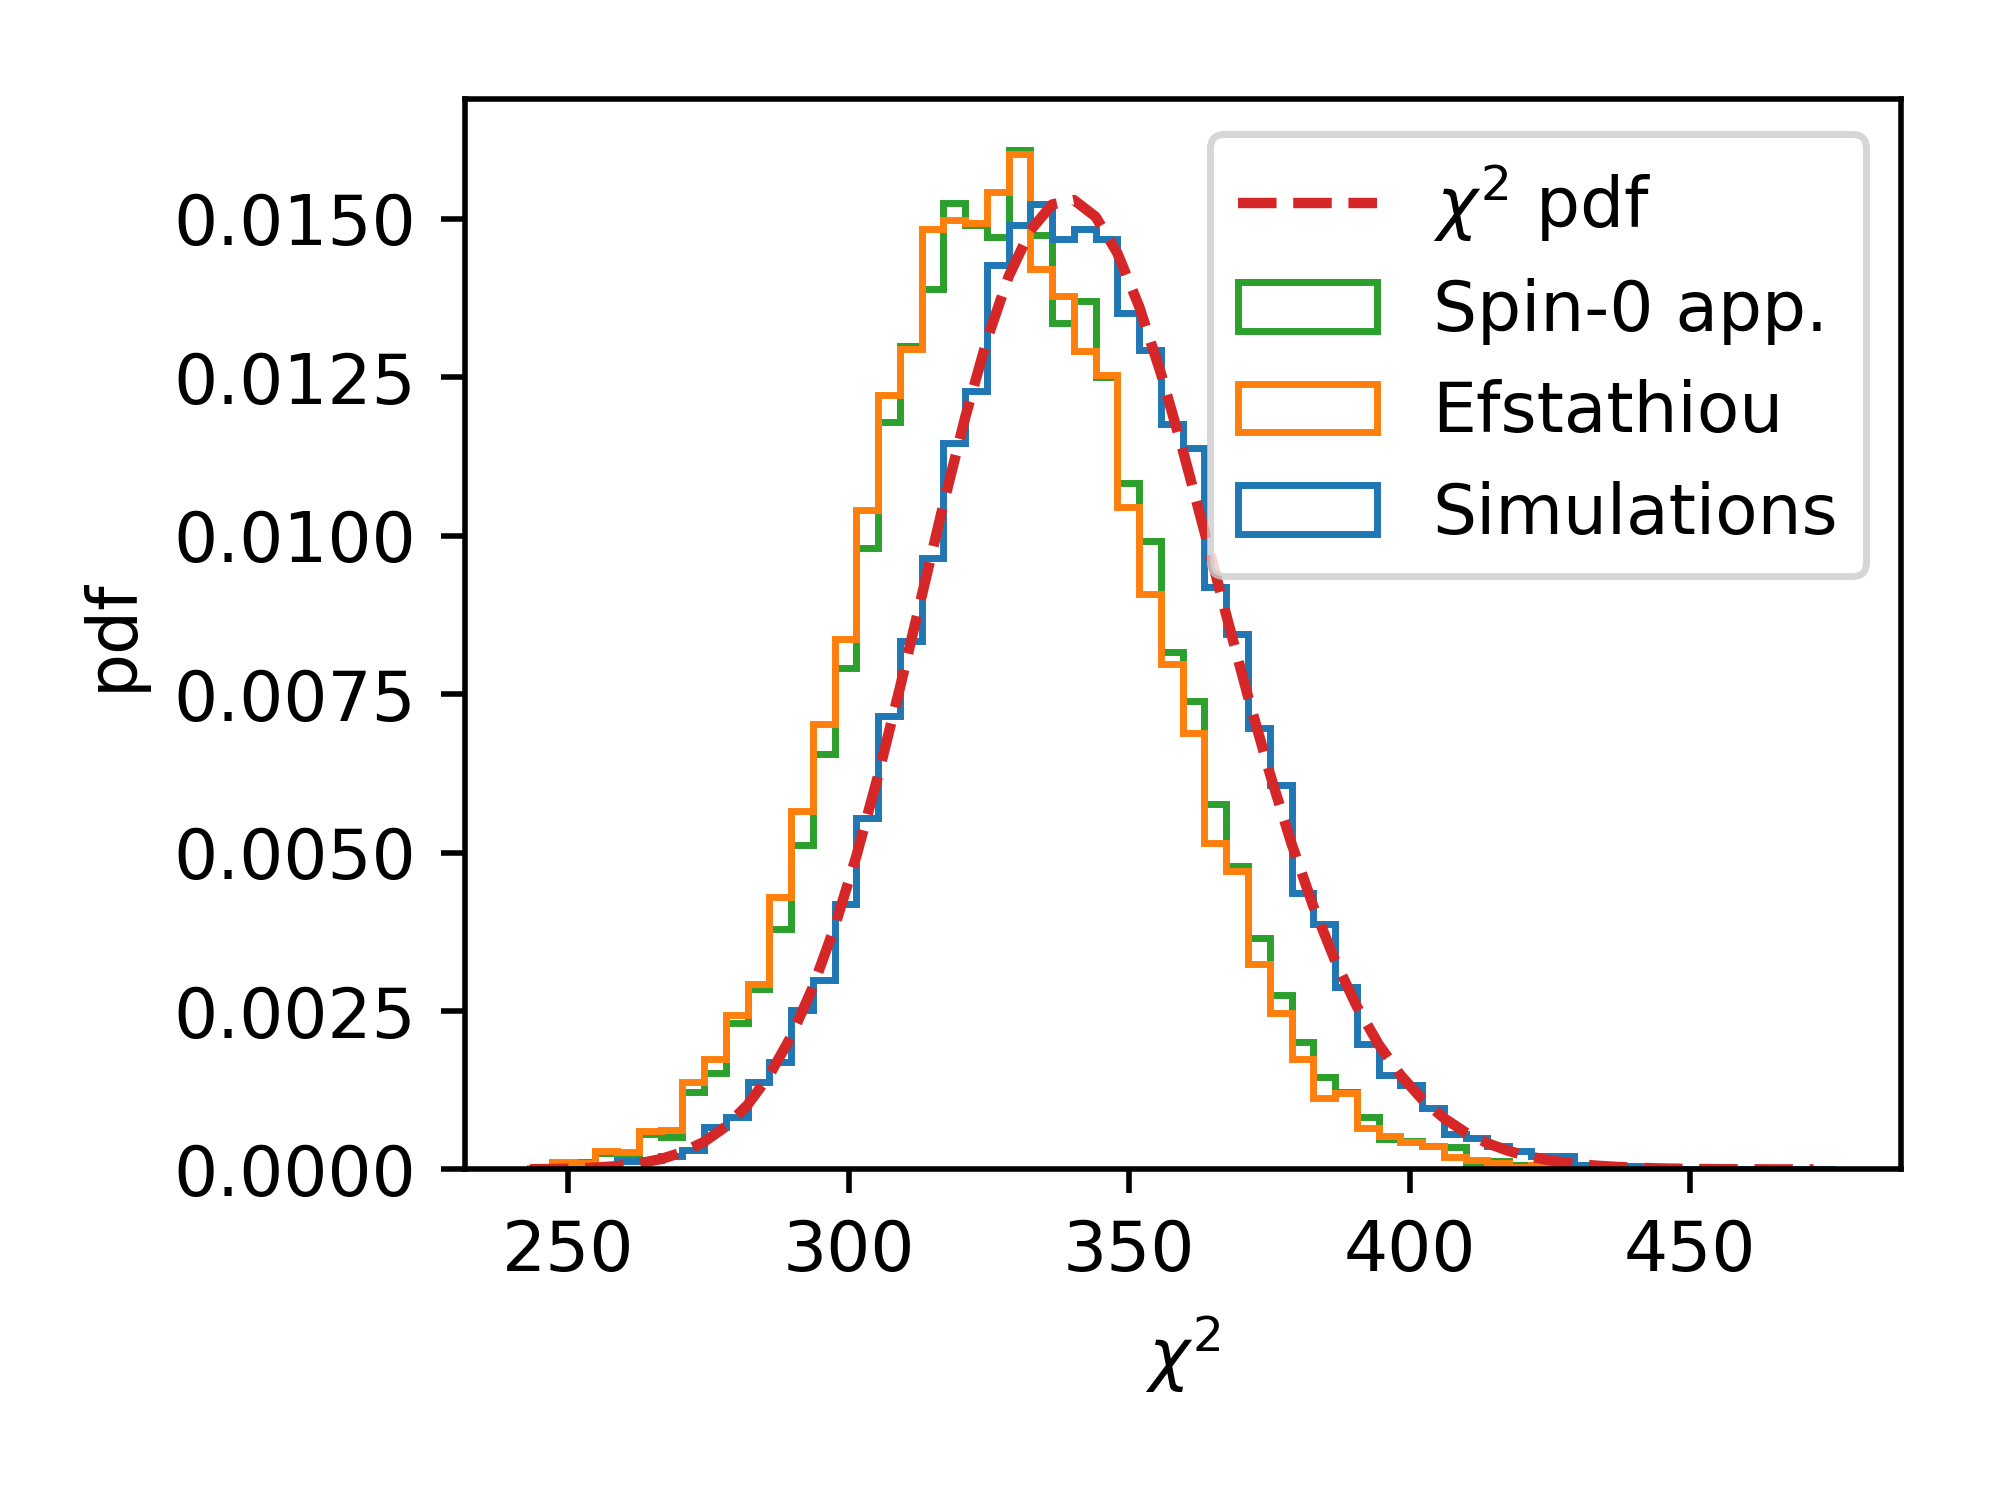
\includegraphics[width=\columnwidth]{./figures/run_sph_ALL_EEEE_chi2.png}
  \caption{Comparison of the distributions found using different
    covariances for the TTTT (left) and EEEE (right) cases.}
  \label{fig:TTTT_EEEE_chi2}
\end{figure*}

\begin{figure*} %[htb]
  \centering
  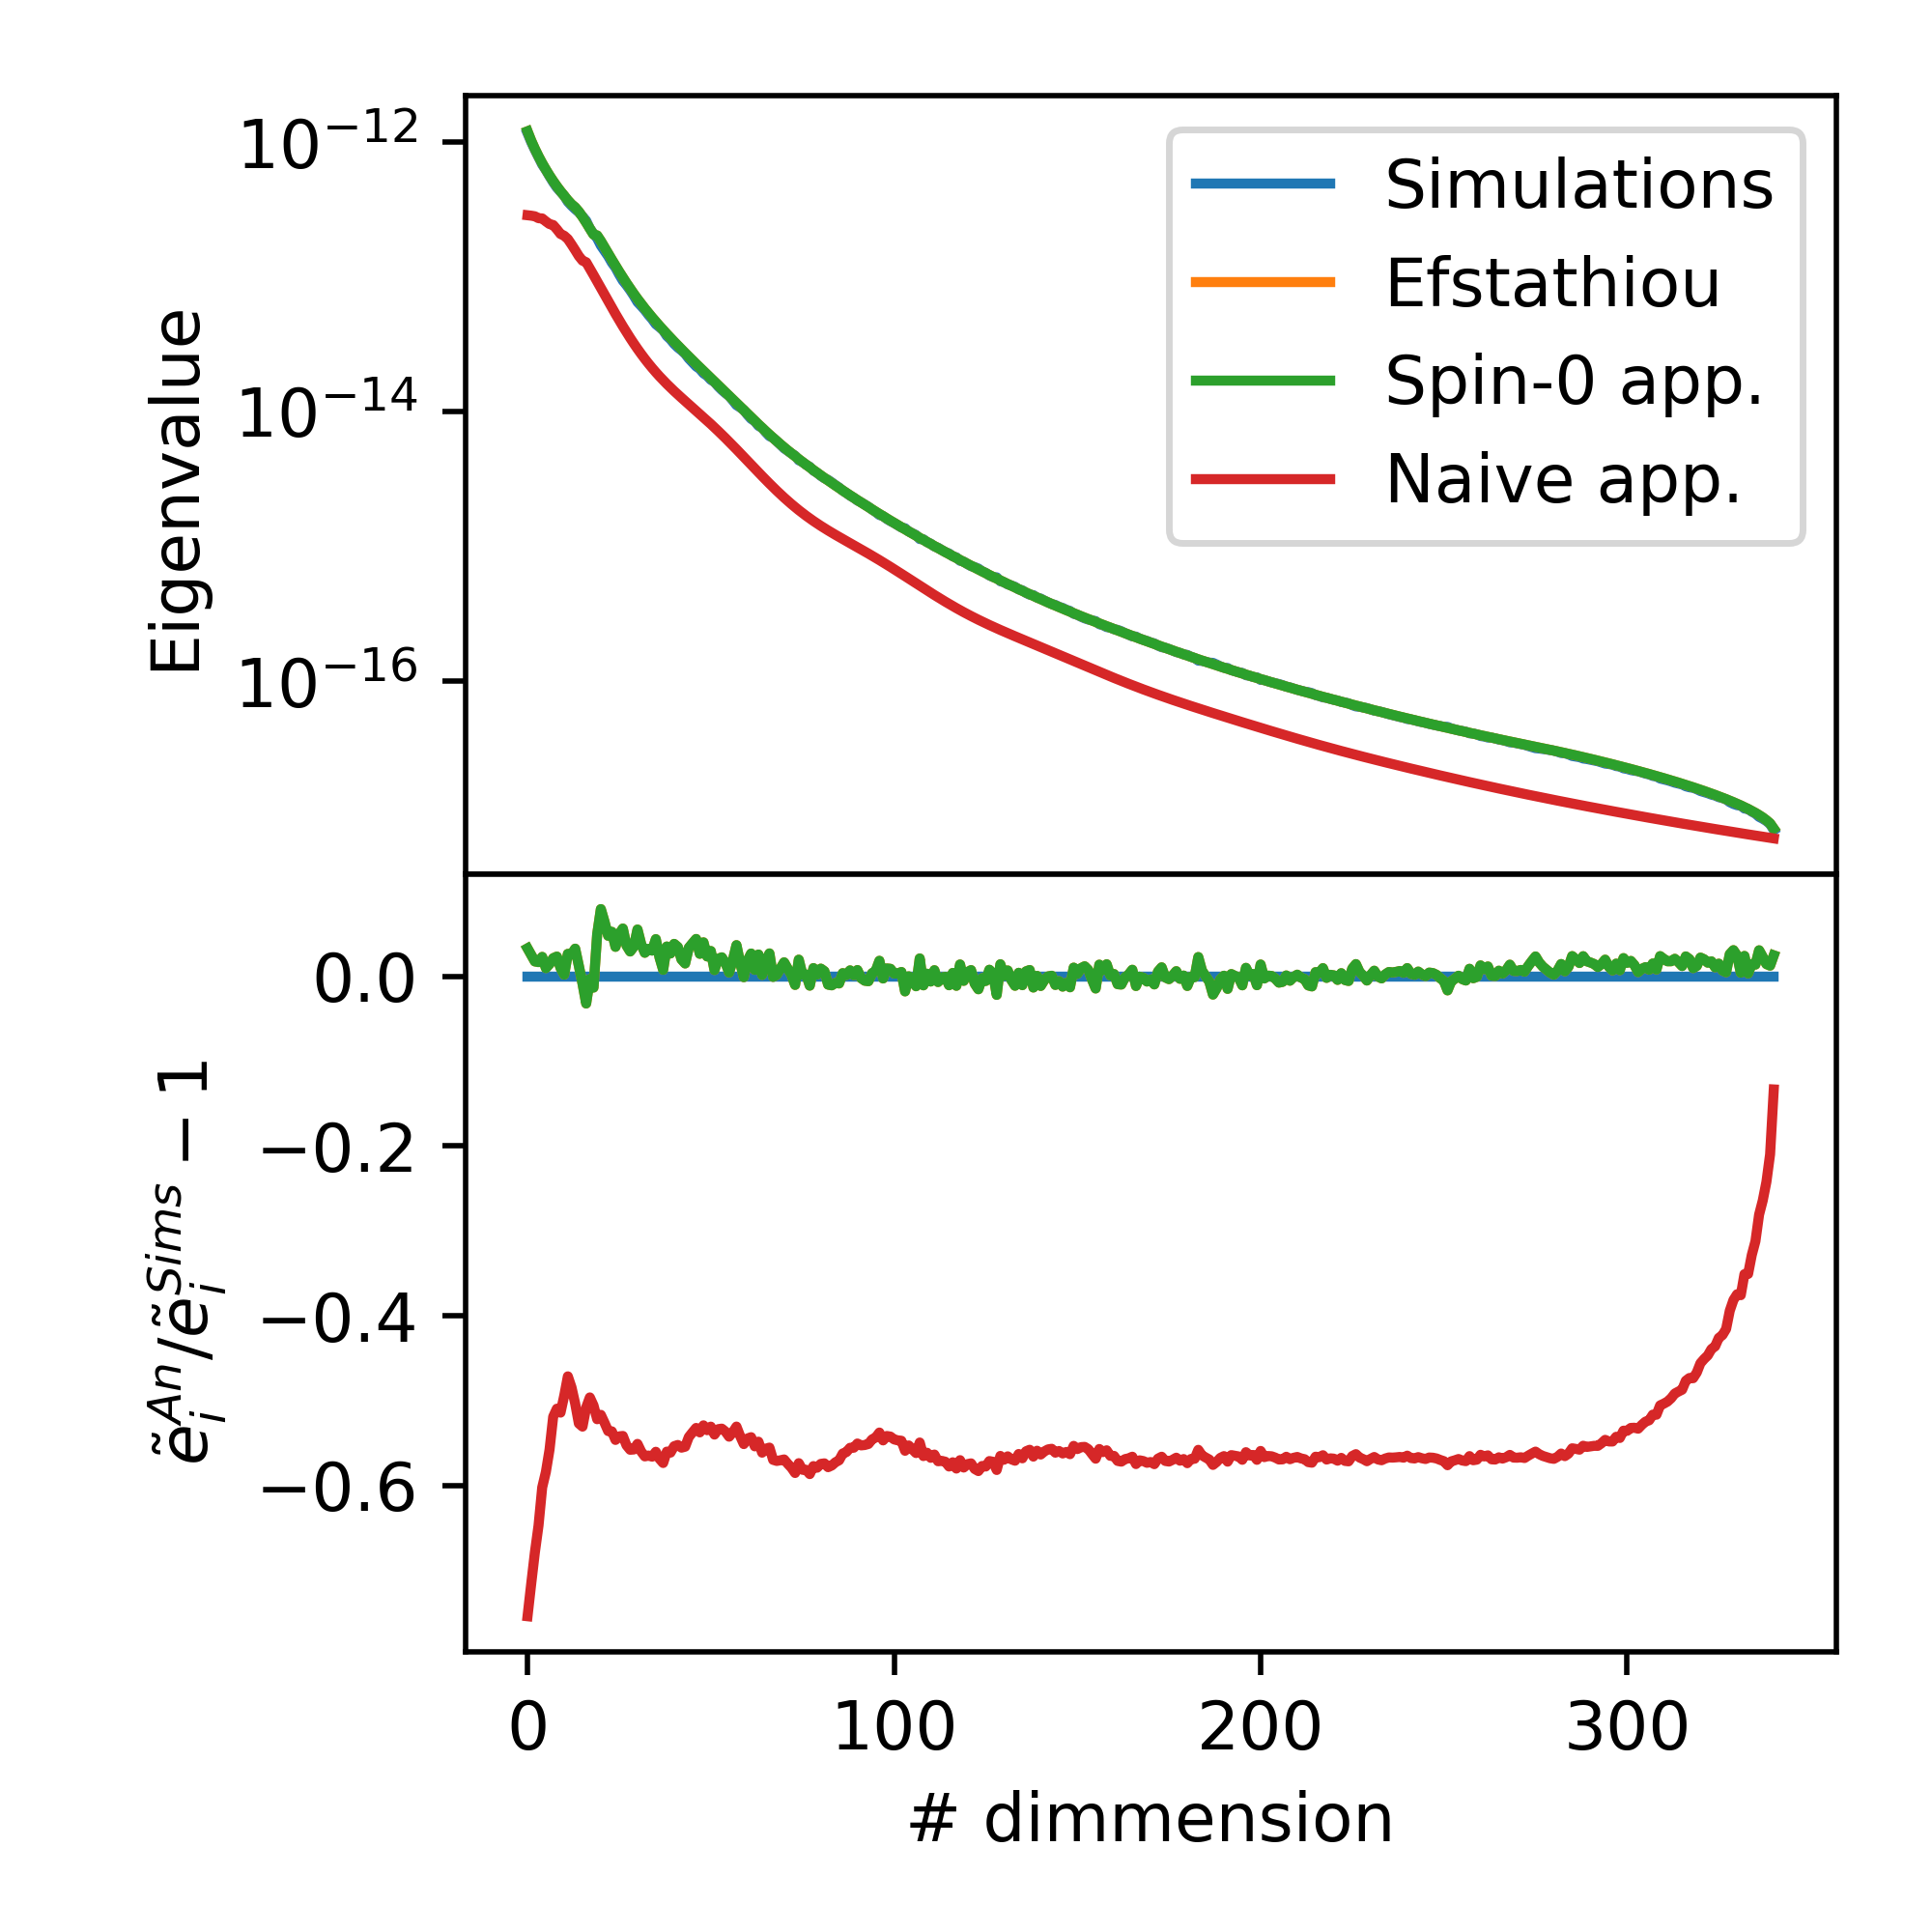
\includegraphics[width=\columnwidth]{./figures/run_sph_ALL_TTTT_reldev_eigval.png}~
  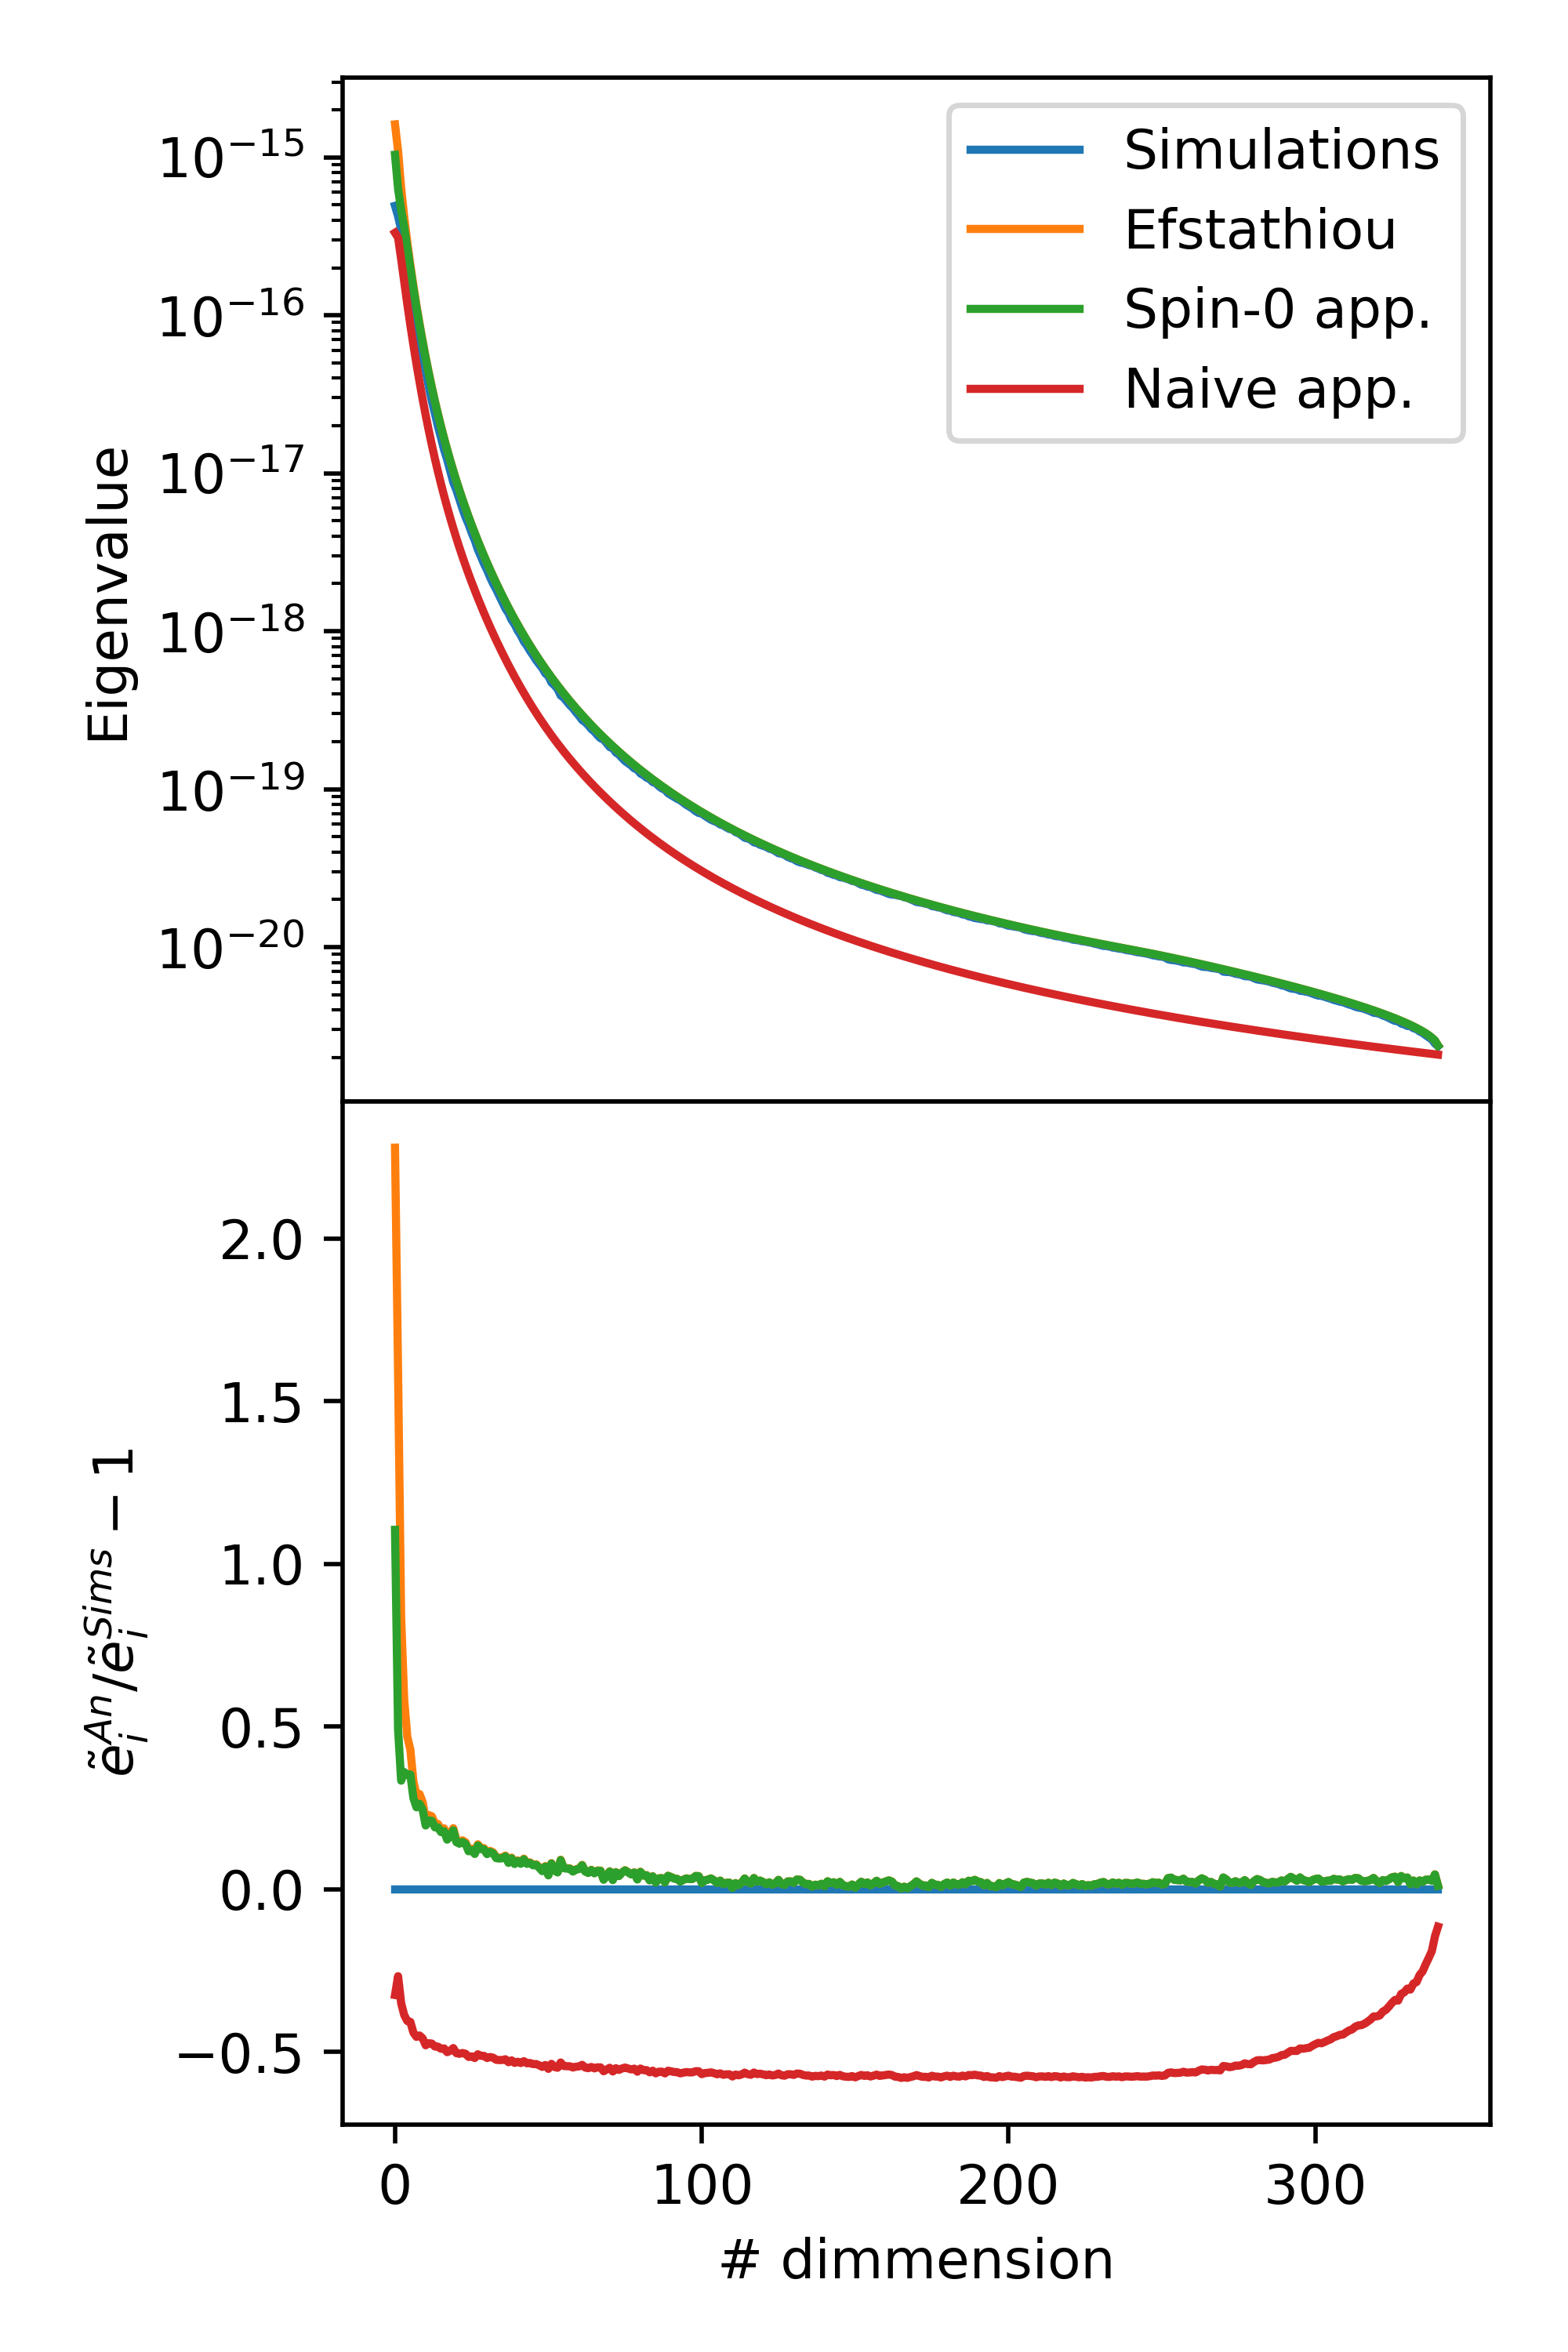
\includegraphics[width=\columnwidth]{./figures/run_sph_ALL_EEEE_reldev_eigval.png}
  \caption{Comparison of the covariance matrix eigenvalues for the TTTT (left)
    and EEEE (right) cases.} 
  \label{fig:TTTT_EEEE_eigv}
\end{figure*}

\begin{figure} %[htb]
  \centering
  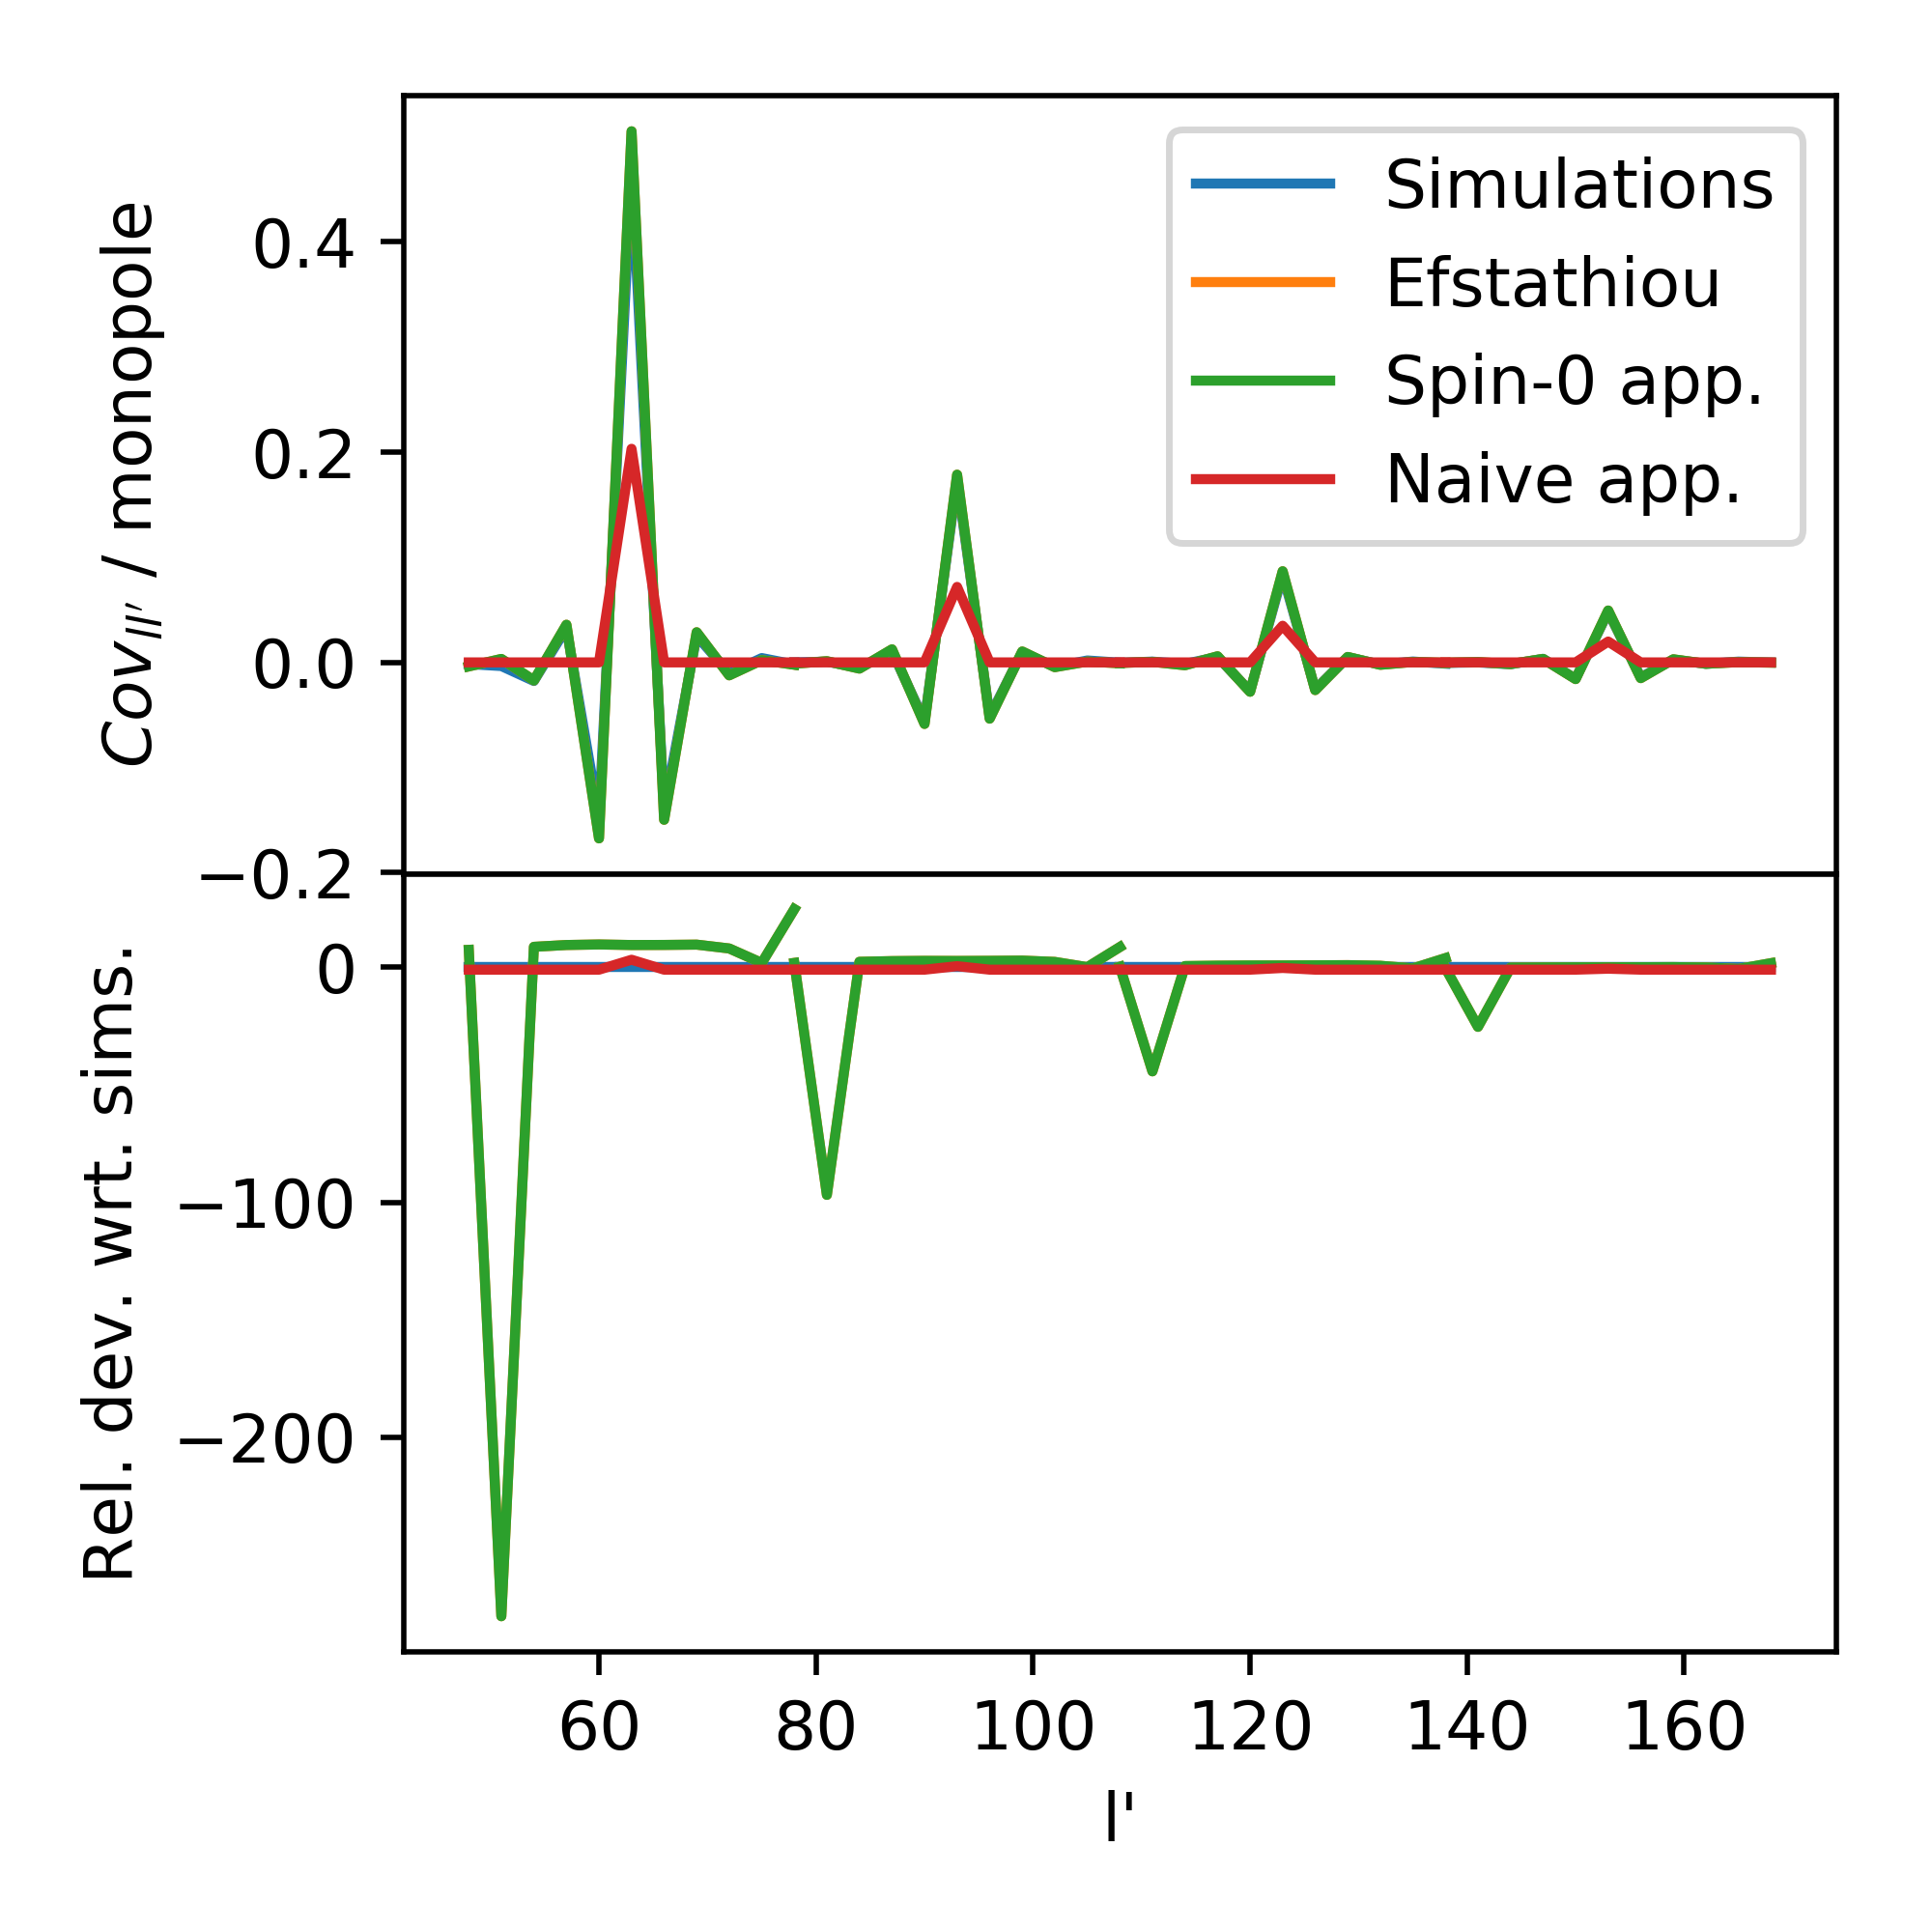
\includegraphics[width=\columnwidth]{./figures/run_sph_ALL_TTTT_rows_cov_matrix.png}~
  \caption{Mask induced scale correlations for the TTTT case.}
  \label{fig:TTTT_rows}
\end{figure}

The goodness of the approximation is also seen in the correlation matrices.
The subtraction of the correlation matrix from the simulations and that from
the best analytical approximation (which we have just seen gives almost same
results as the spin-0 one) shows no structure but for the case of the larger
scales of the EEEE modes (see Fig.~\ref{fig:TTTT_EEEE_corr}).

\begin{figure*} %[htb]
  \centering
  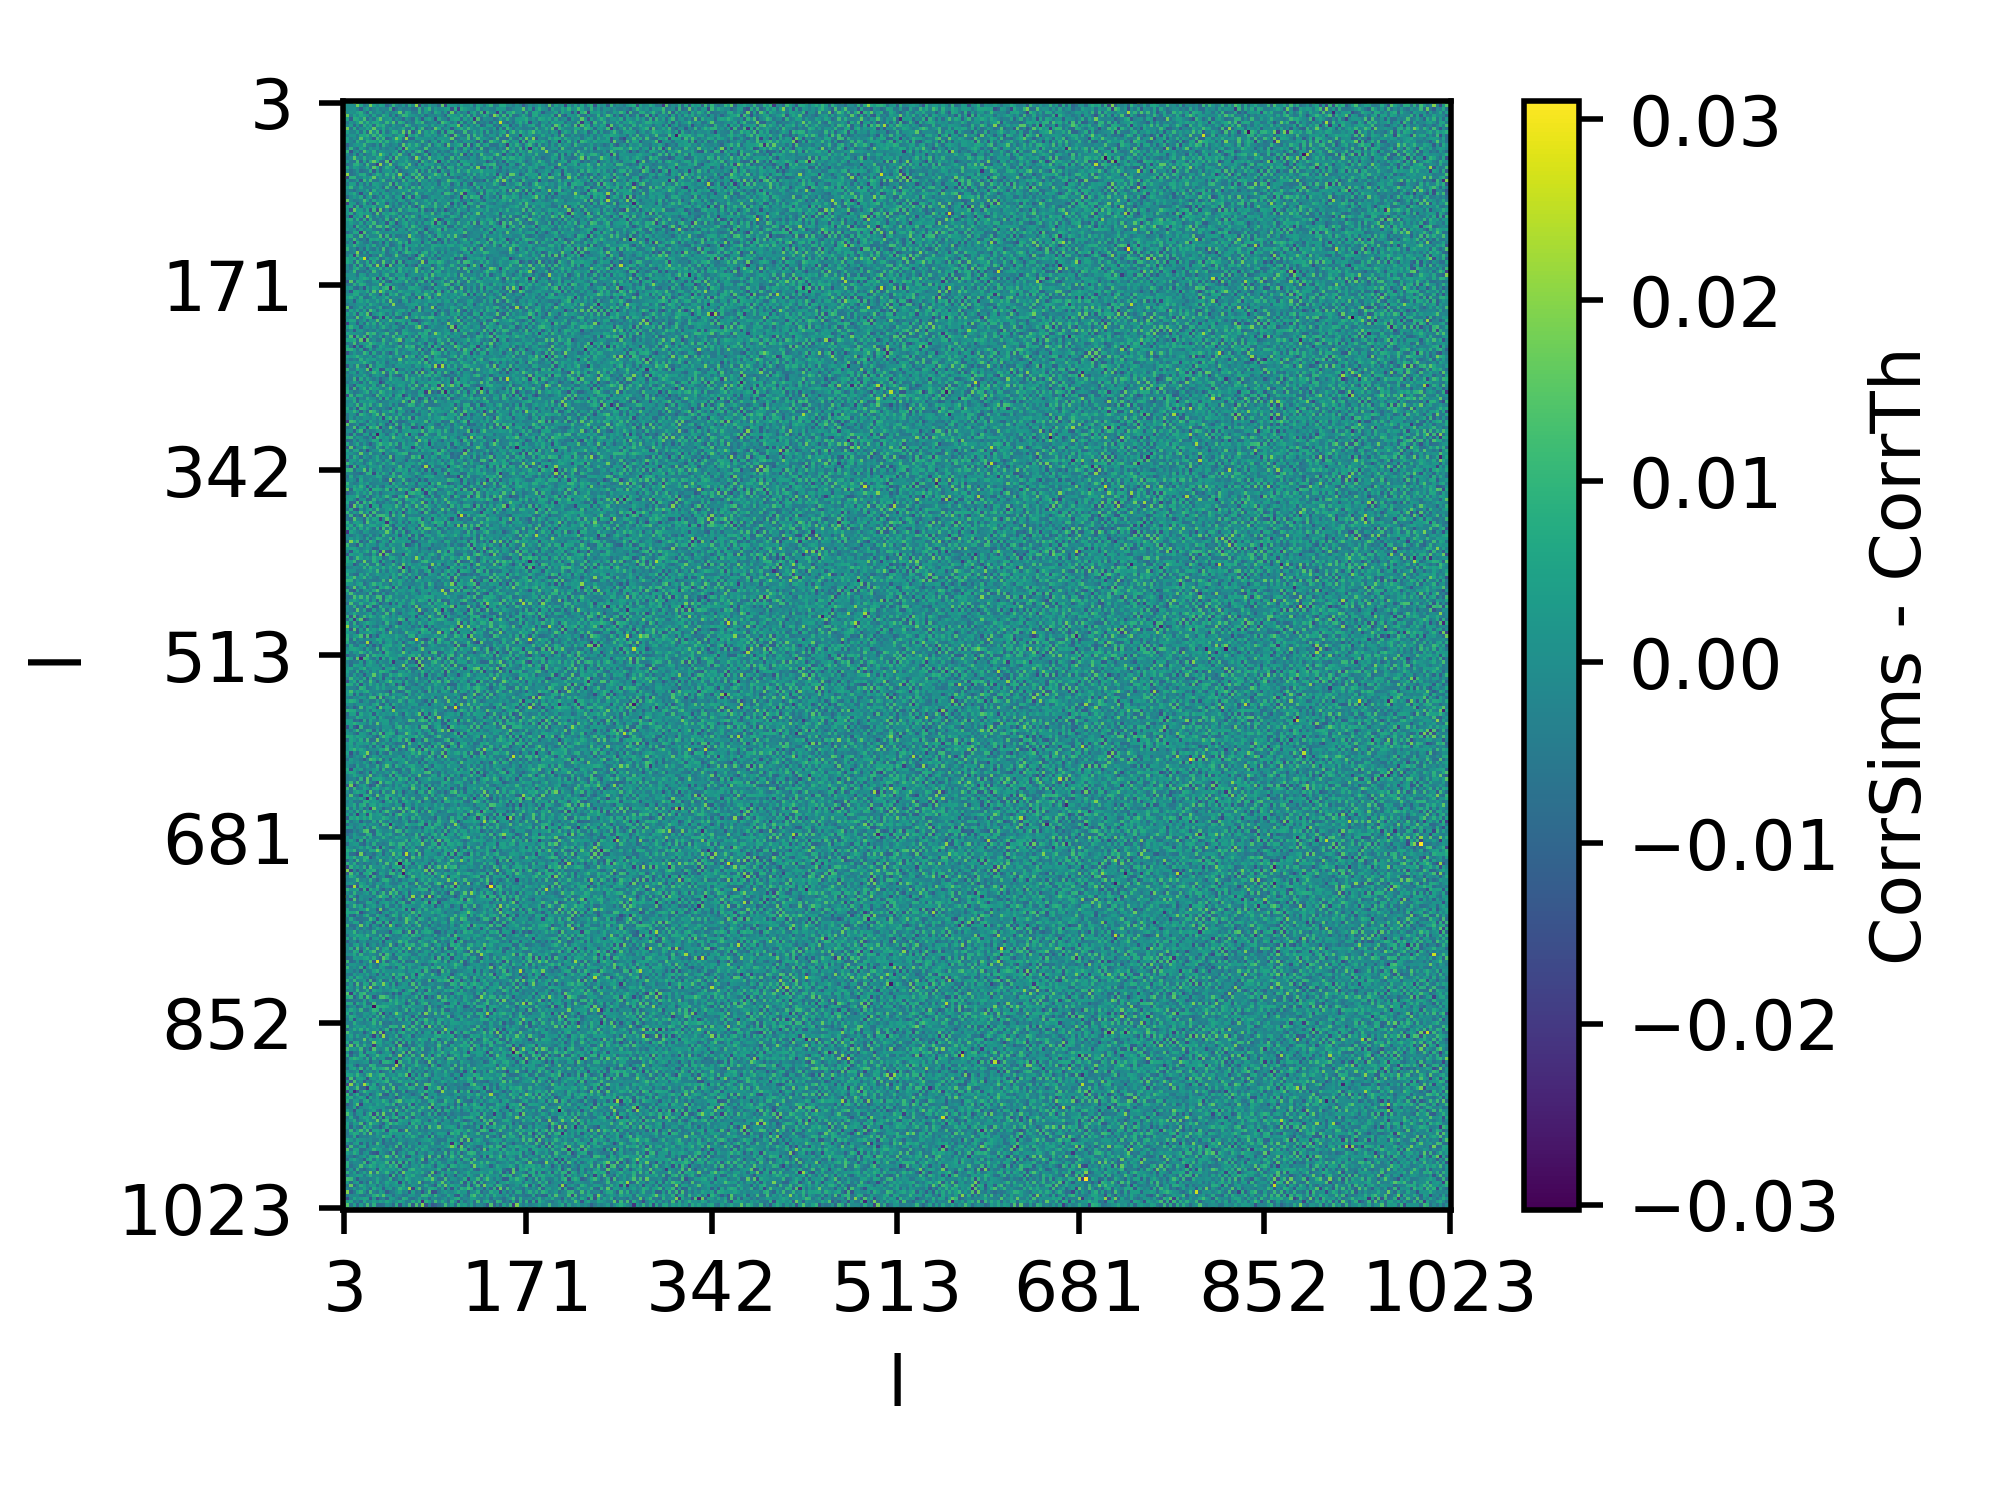
\includegraphics[width=\columnwidth]{./figures/run_sph_Efstathiou_TTTT_correlation_difference.png}~
  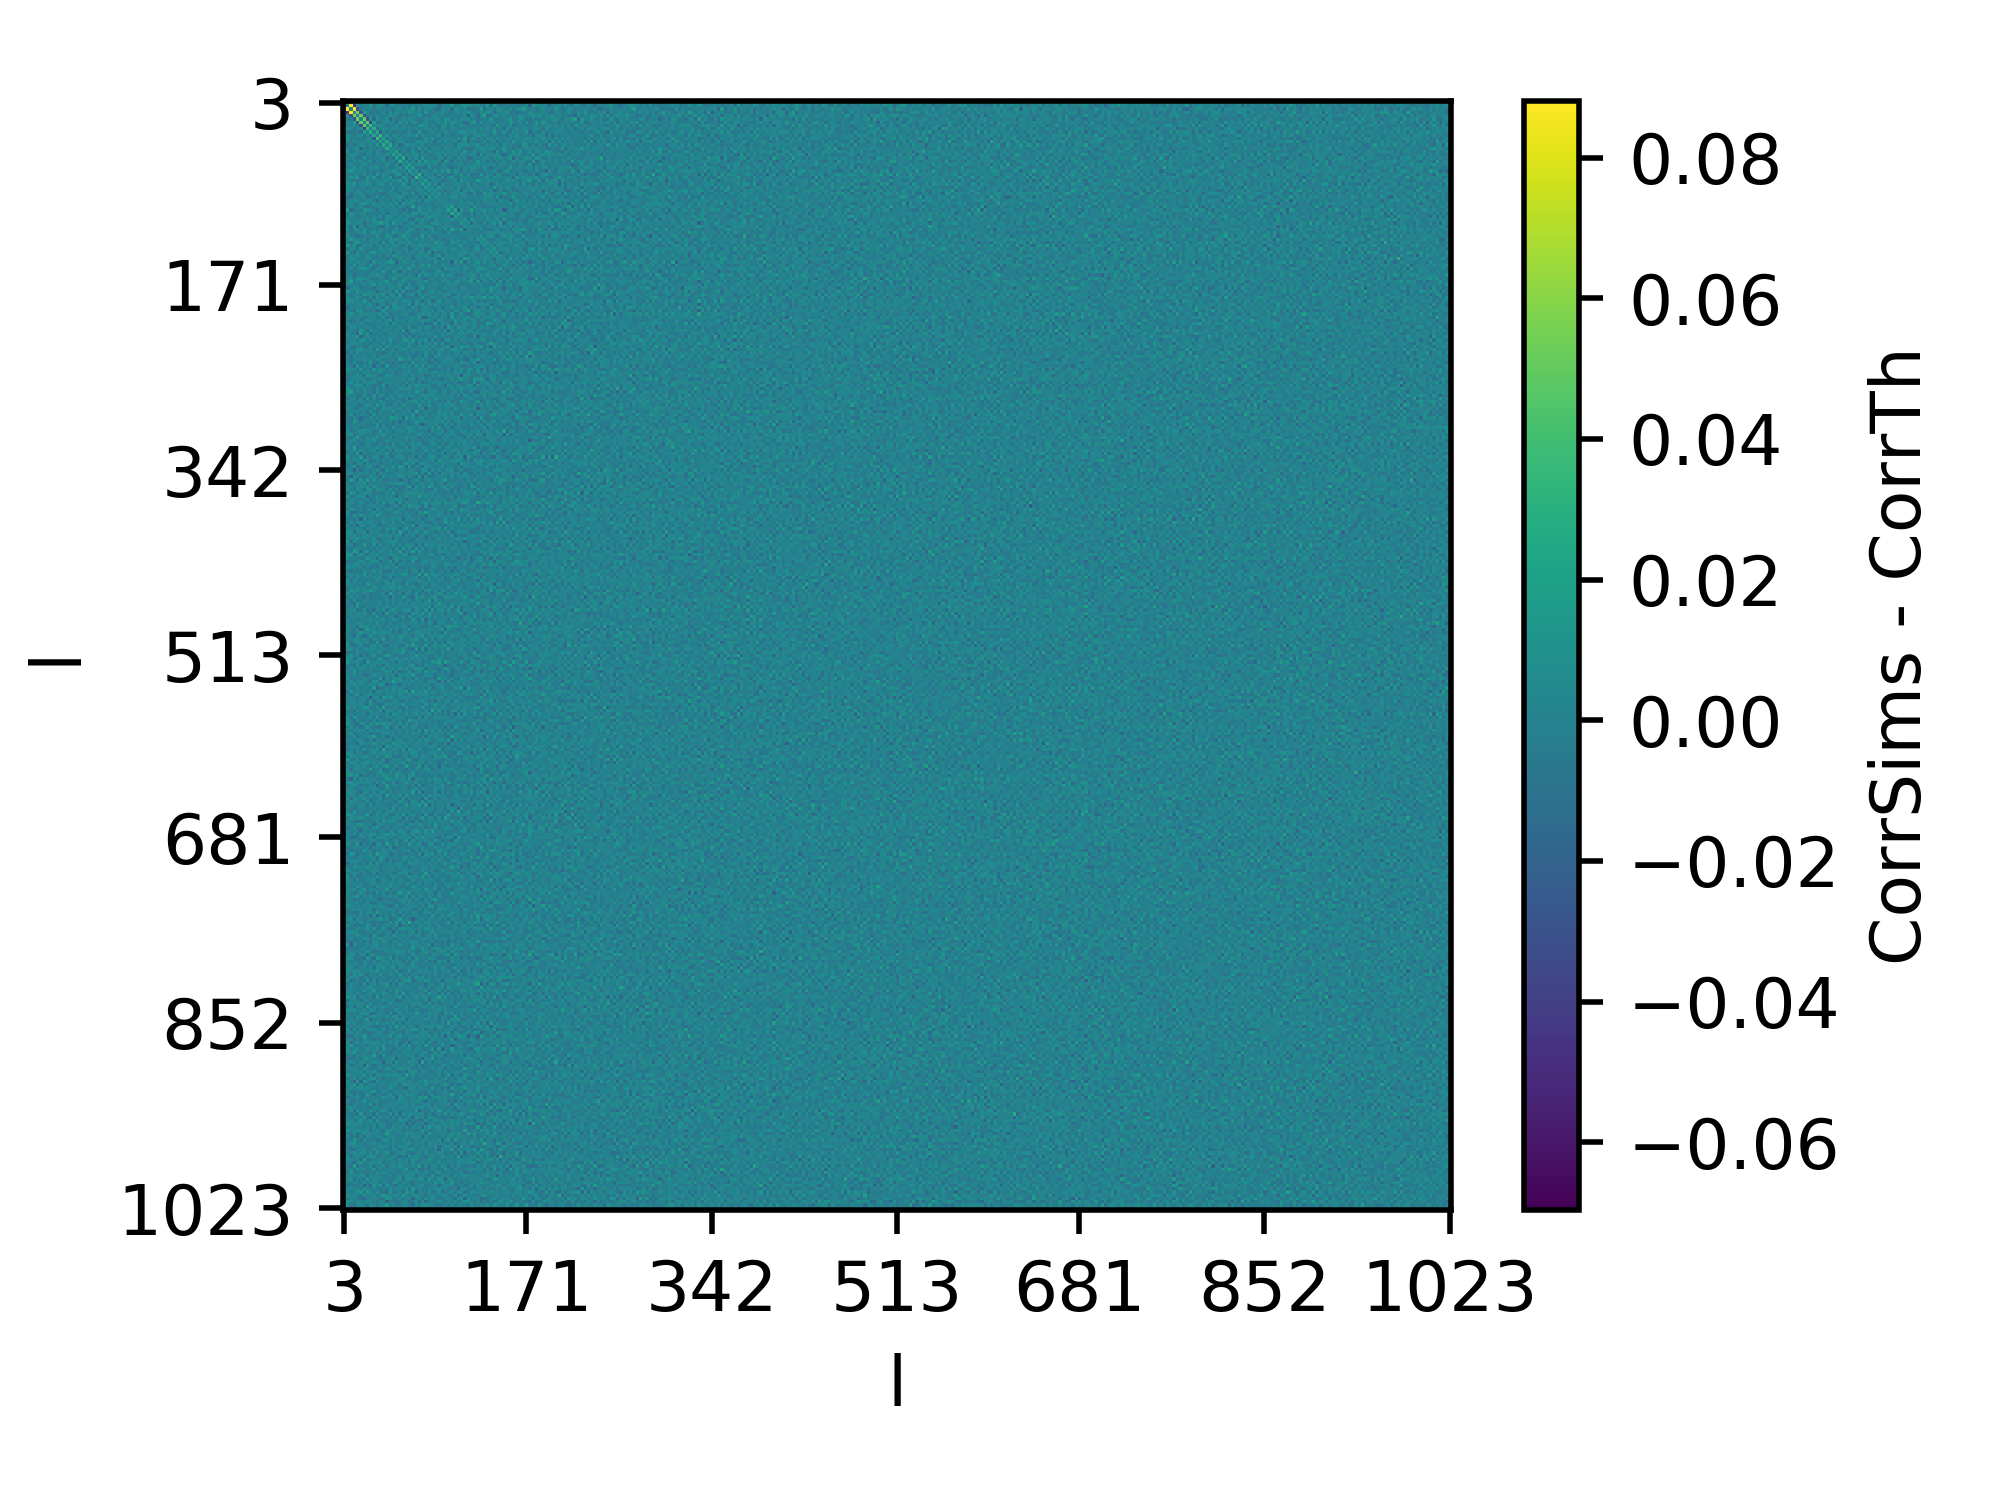
\includegraphics[width=\columnwidth]{./figures/run_sph_Efstathiou_EEEE_correlation_difference.png}
  \caption{Differences between the simulations and analytical approximation of
    the correlation matrices for the TTTT (left) and EEEE (right) cases.}
  \label{fig:TTTT_EEEE_corr}
\end{figure*}

These approximations do not work well for the B-modes, though. We can see in
Fig.~\ref{fig:BBBB} that we are not able to recover with accuracy the first
diagonal elements.


\begin{figure} %[htb]
  \centering
  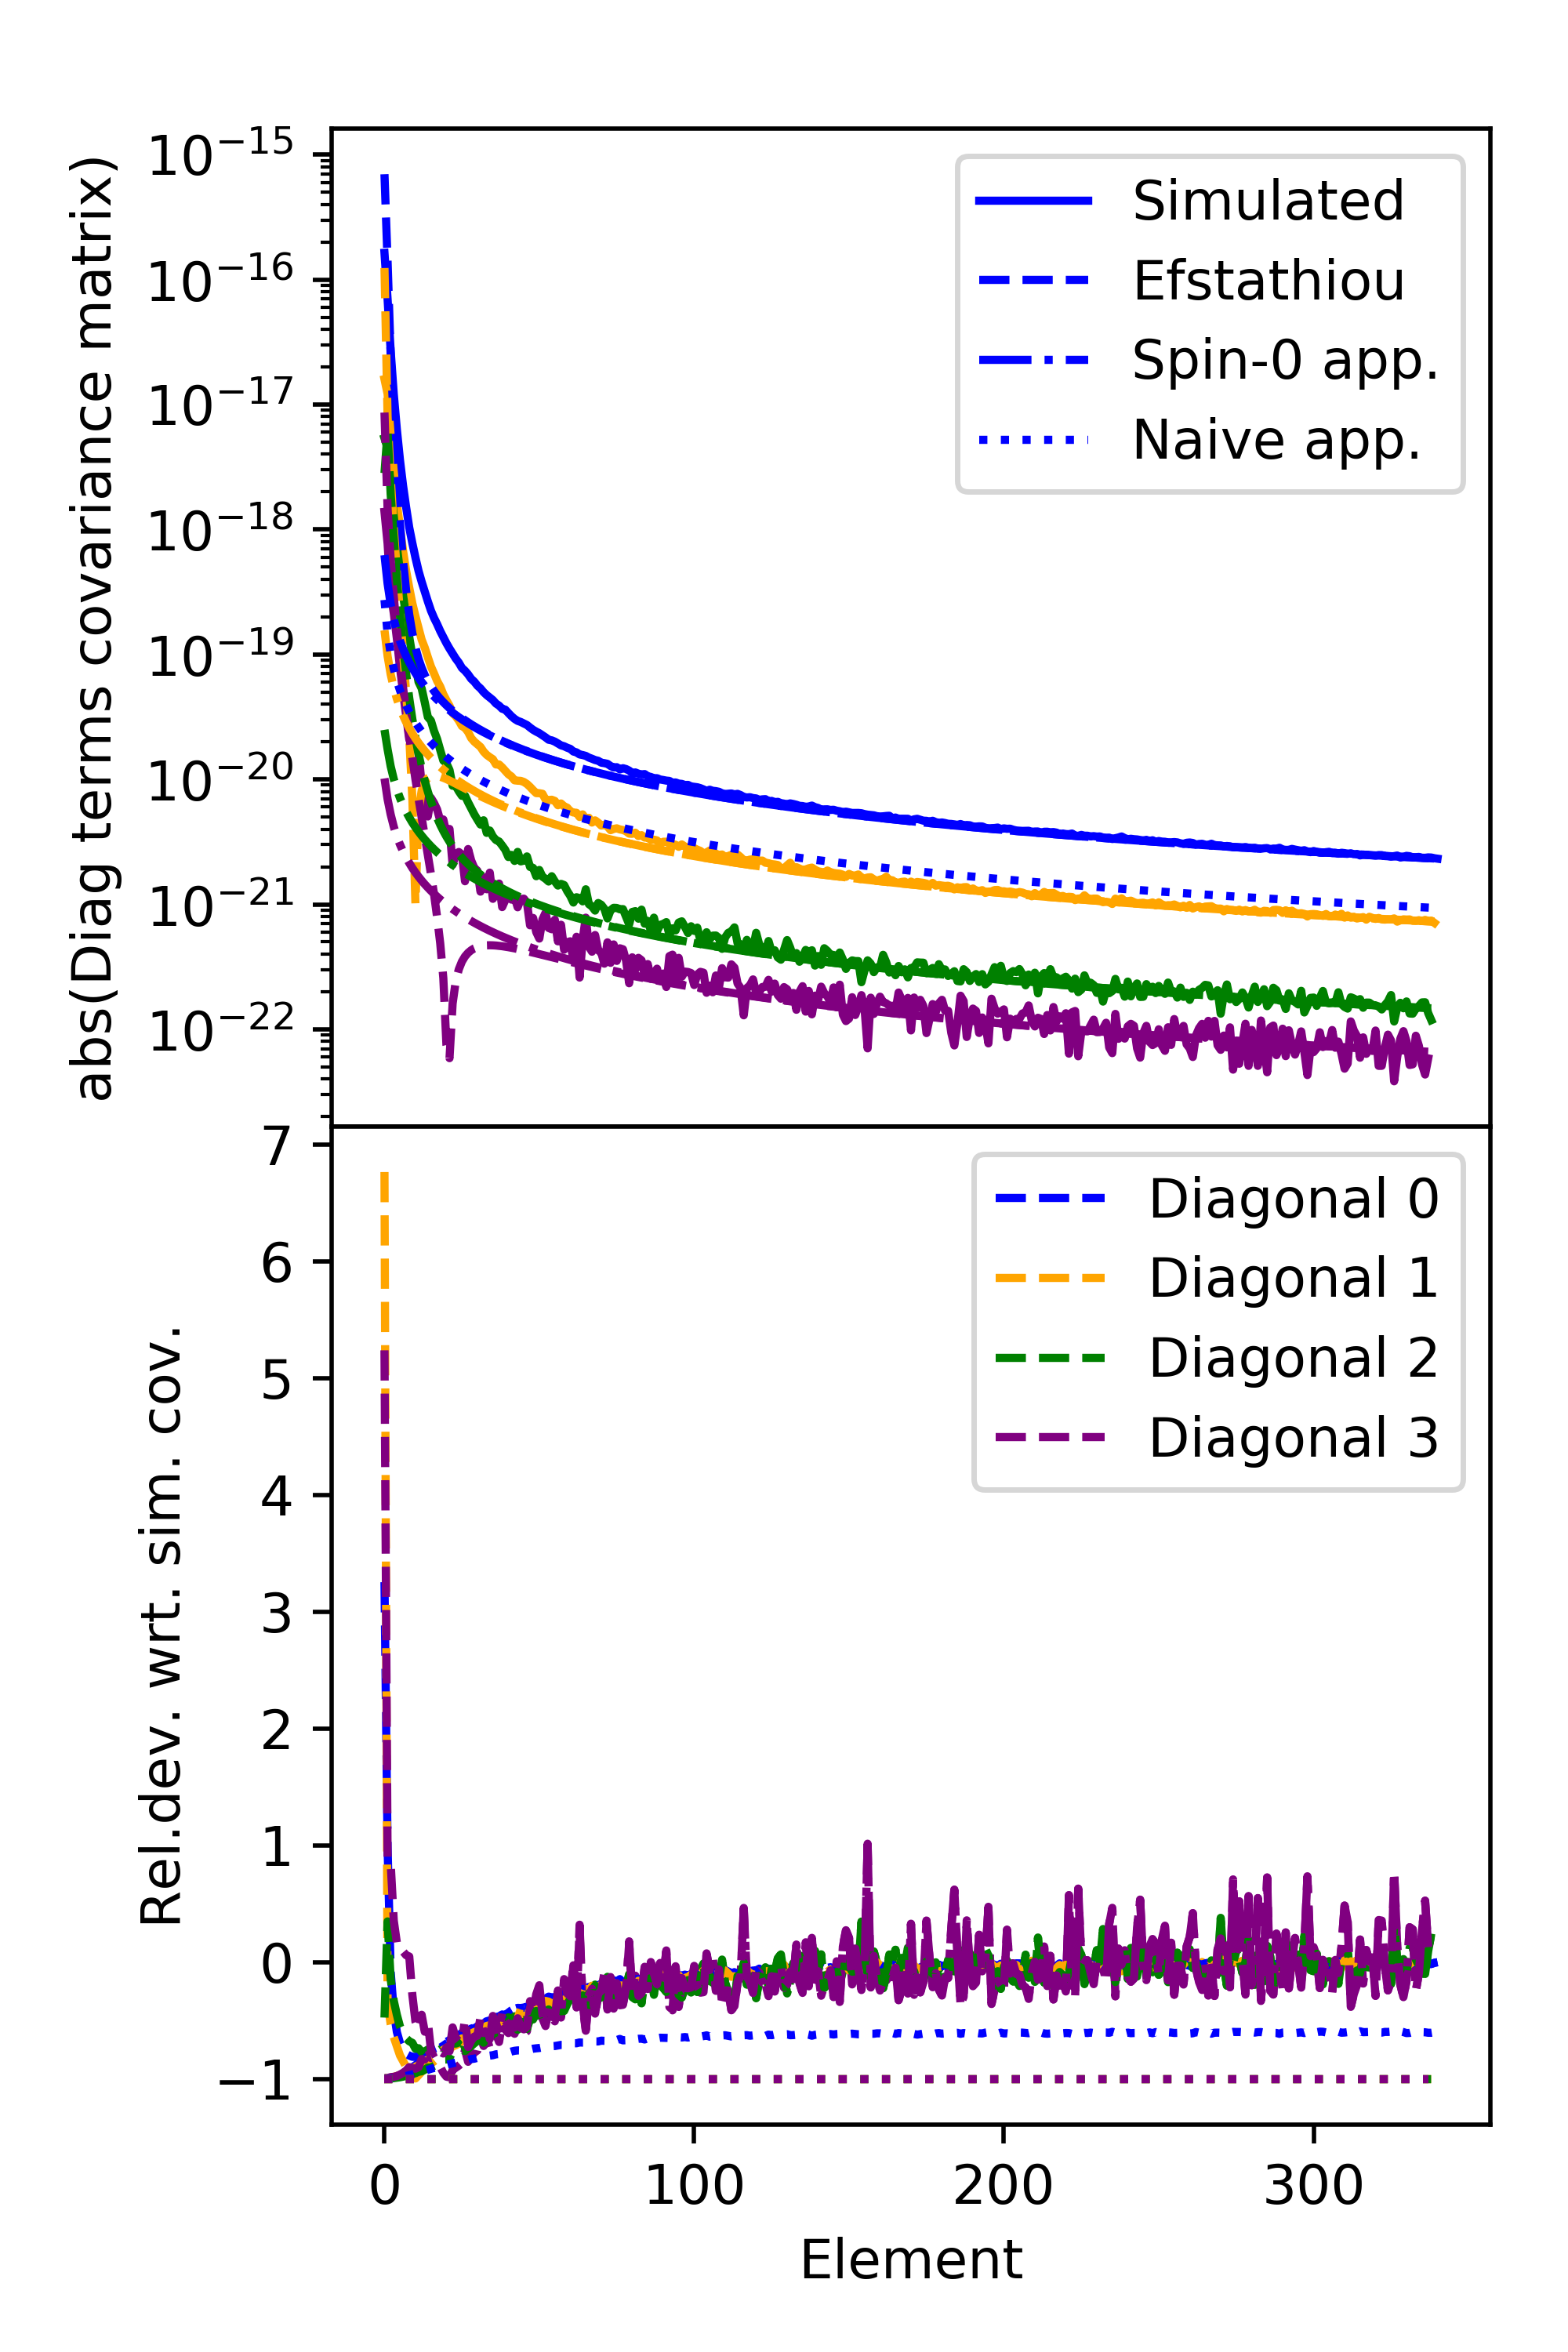
\includegraphics[width=\columnwidth]{./figures/run_sph_ALL_BBBB_check_diagonal_terms_4.png}
  \caption{The analytical approximation are not able to reproduce accurately
    the terms involving the B-modes. Here we show the most extreme case, the
    corresponding to the BBBB modes.}
  \label{fig:BBBB}
\end{figure}

Finally, the analytical covariance also works for 2-bin correlations. The
$\chi^2$ distribution for the covariance matrix of the modes TT, TE and EE
among two bins is shown in Fig.~\ref{fig:TTTEEE_chi2}. The eigenvalues
are recovered well except for the lower ones that diverge up to $20\%$ (see
Fig.~\ref{fig:TTTEEE_eigv}, this is not translated to any substantial
difference in the correlation matrices (see Fig.~\ref{fig:TTTEEE_corr}).

\begin{figure} %[htb]
  \centering
  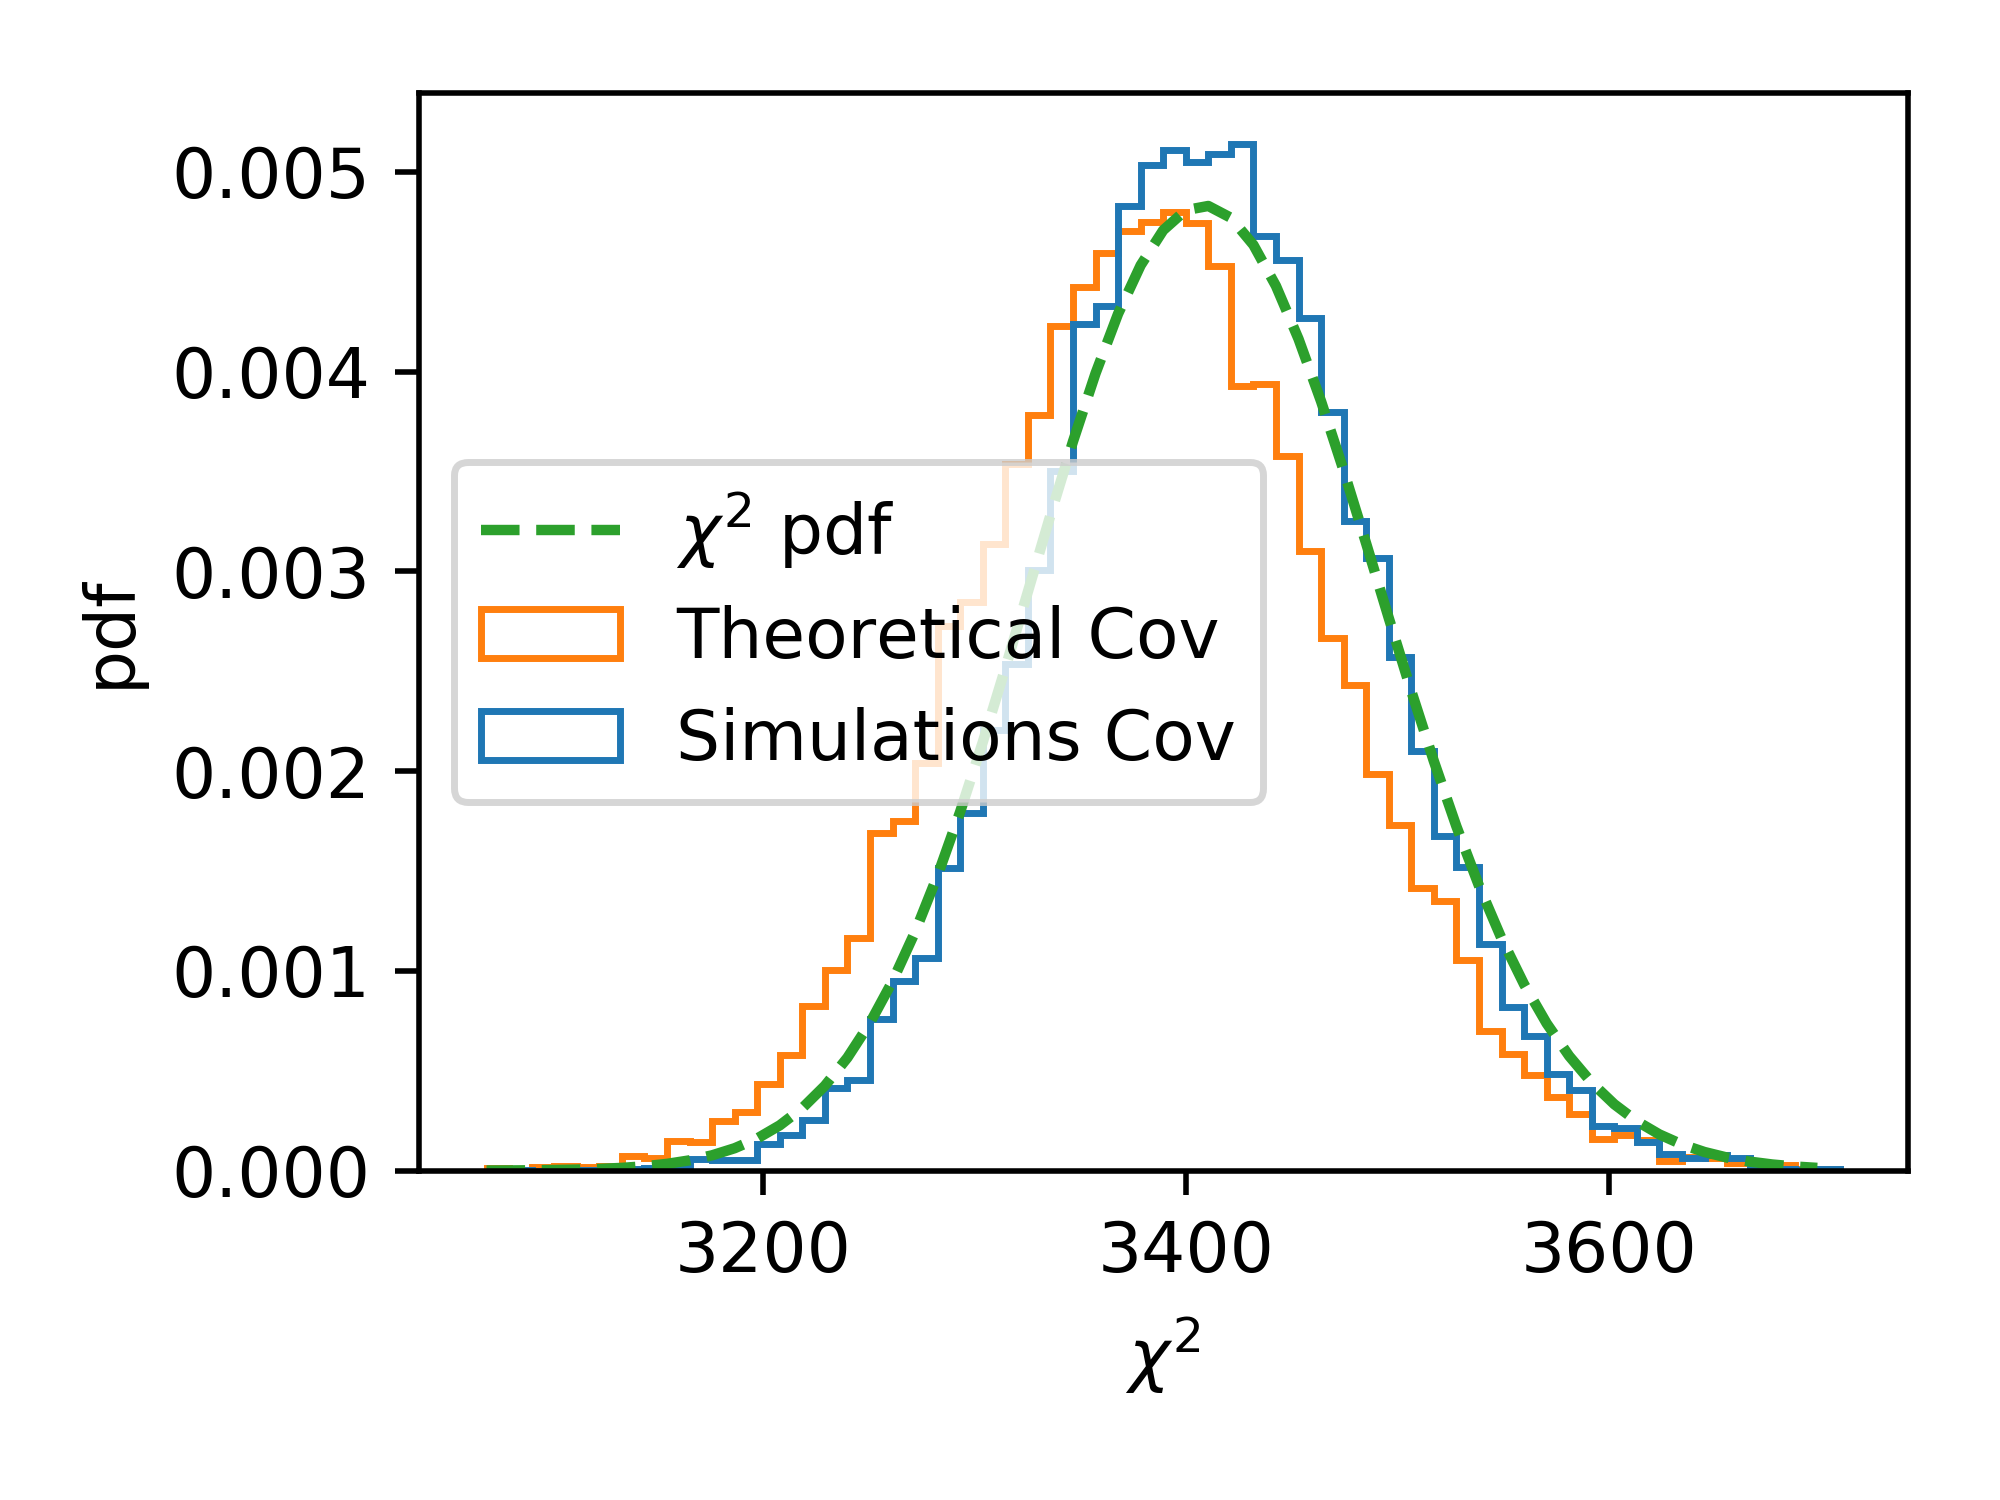
\includegraphics[width=\columnwidth]{./figures/run_sph_2b_same_mask_Efstathiou_TTTEEE_Full_chi2.png}
  \caption{$\chi^2$ distribution check for the full analytical covariance
    matrix for the modes TT, TE and EE among two bins.}
  \label{fig:TTTEEE_chi2}
\end{figure}

\begin{figure} %[htb]
  \centering
  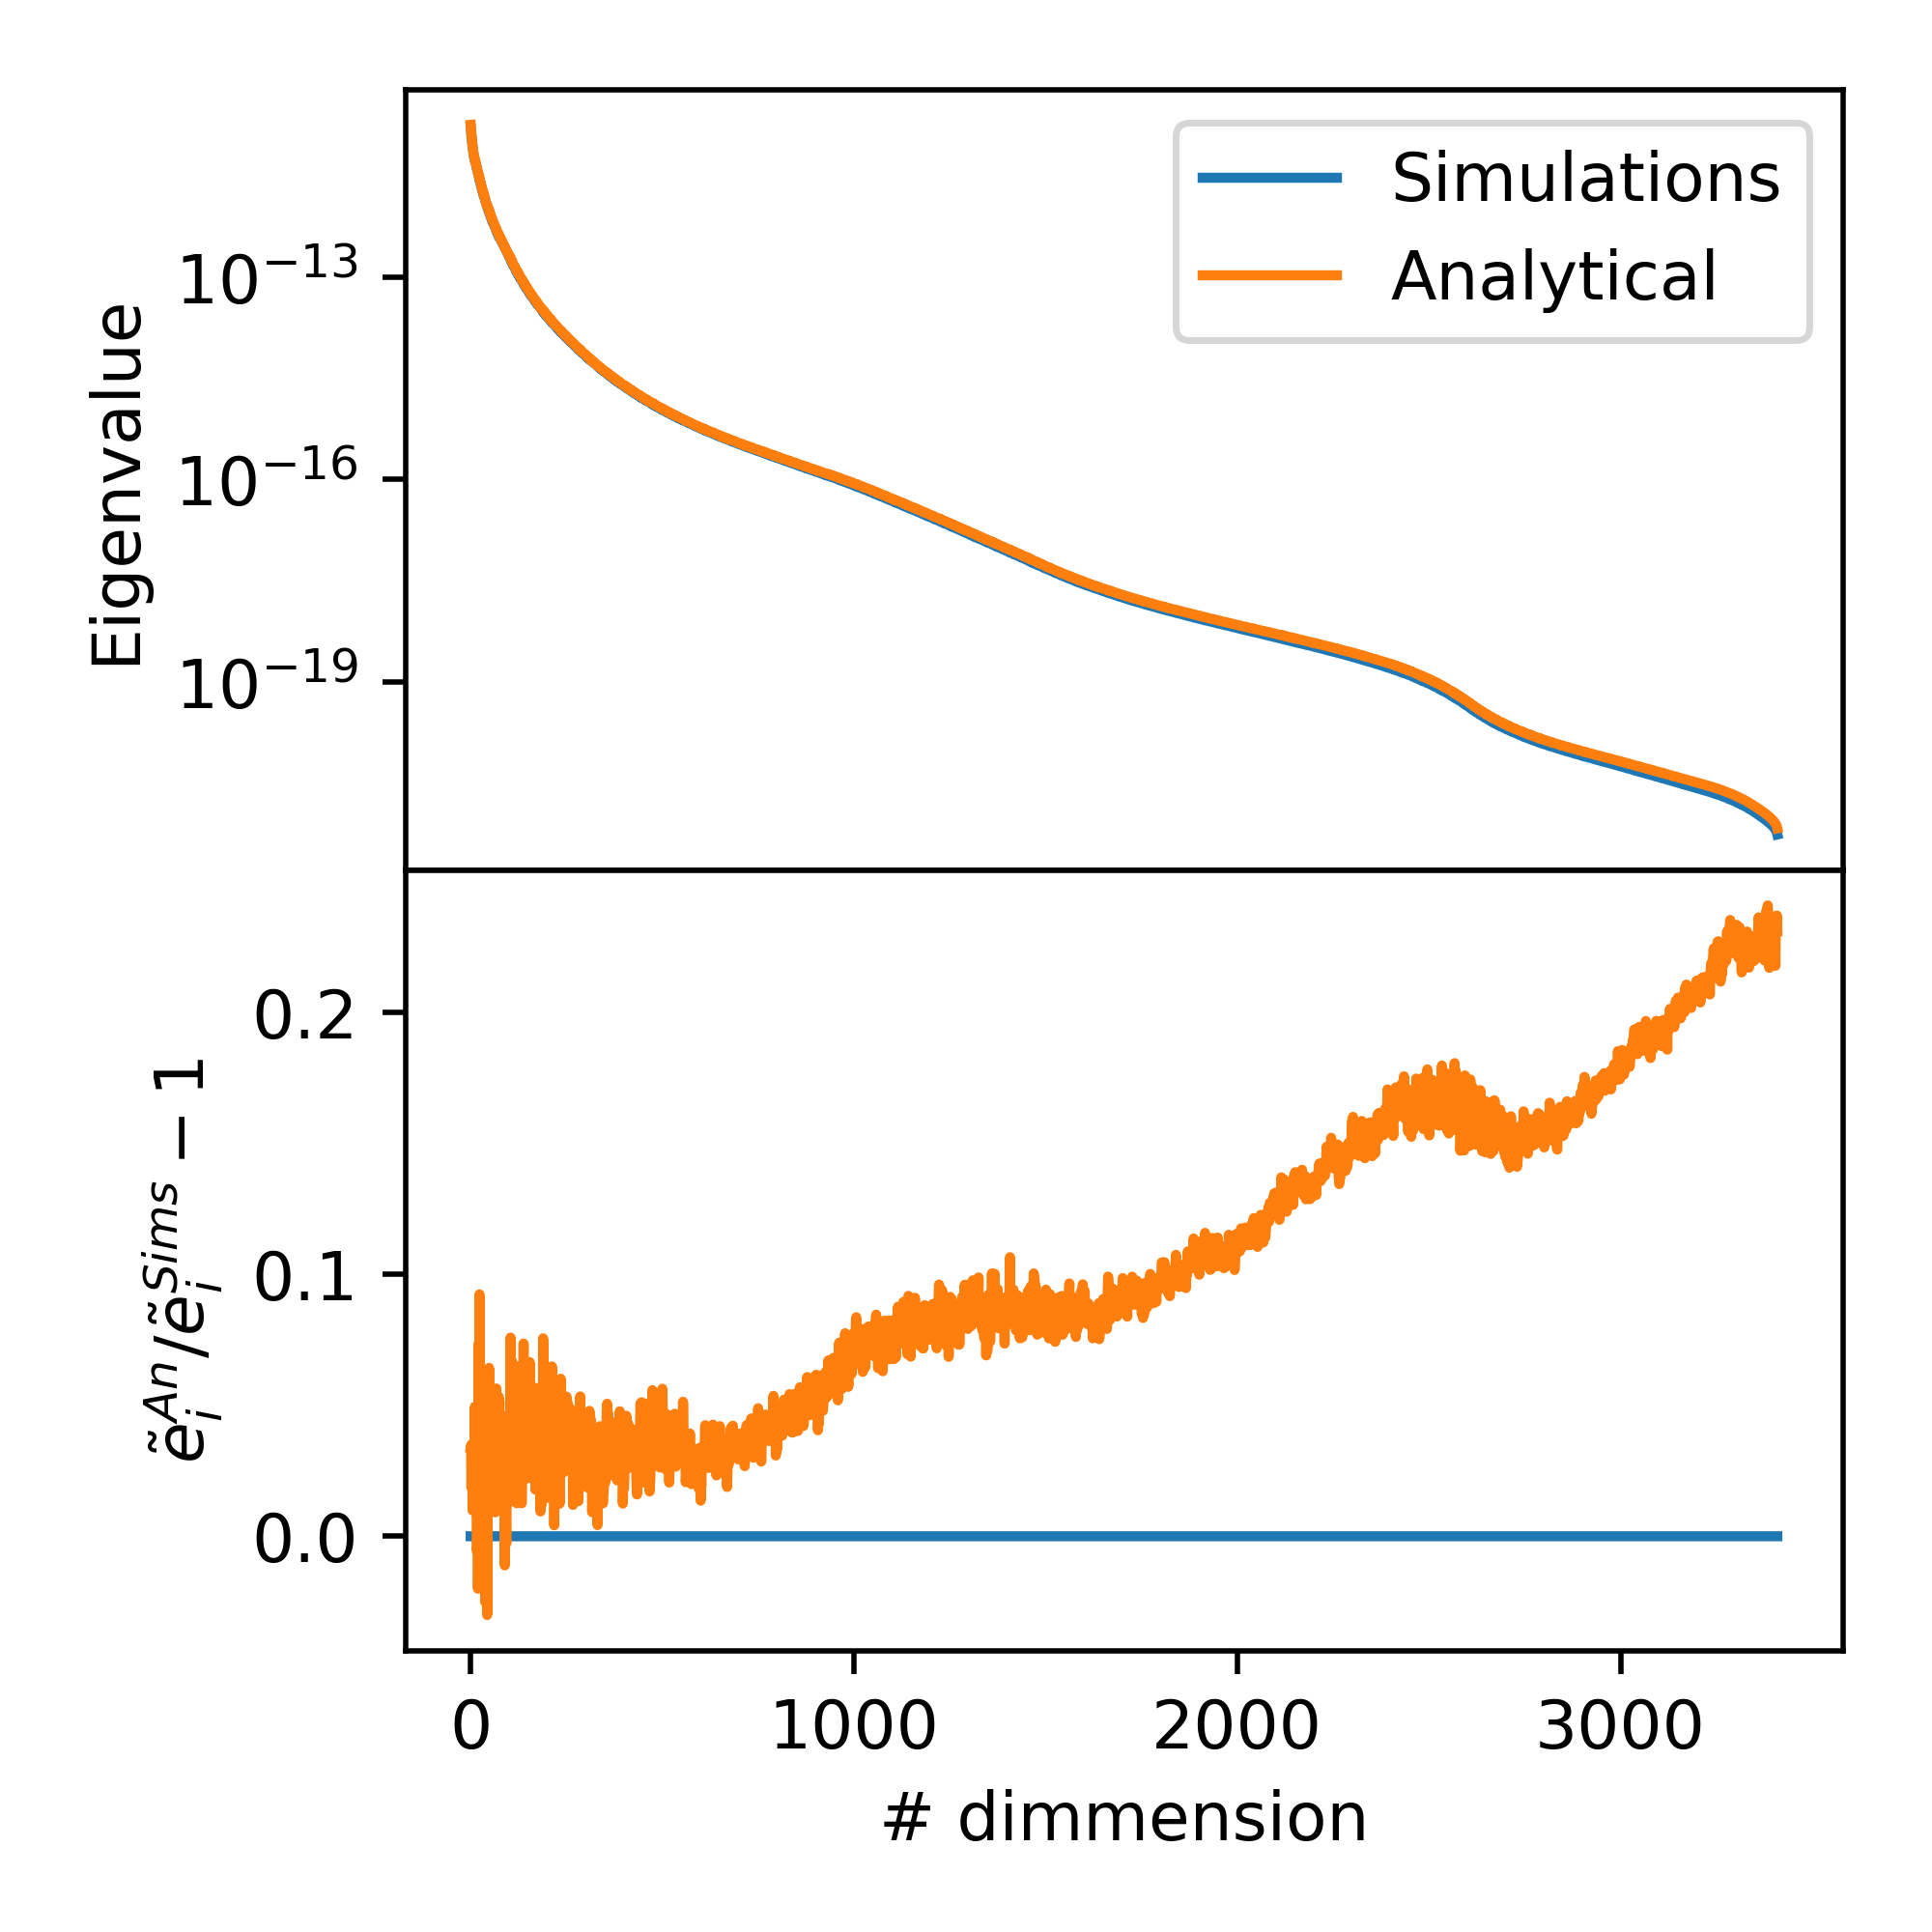
\includegraphics[width=\columnwidth]{./figures/run_sph_2b_same_mask_Efstathiou_TTTEEE_Full_reldev_eigval.png}
  \caption{Relative difference between the analytical and simulations
    covariance matrix eigenvalues for the modes TT, TE and EE among two bins.}
  \label{fig:TTTEEE_eigv}
\end{figure}

\begin{figure} %[htb]
  \centering
  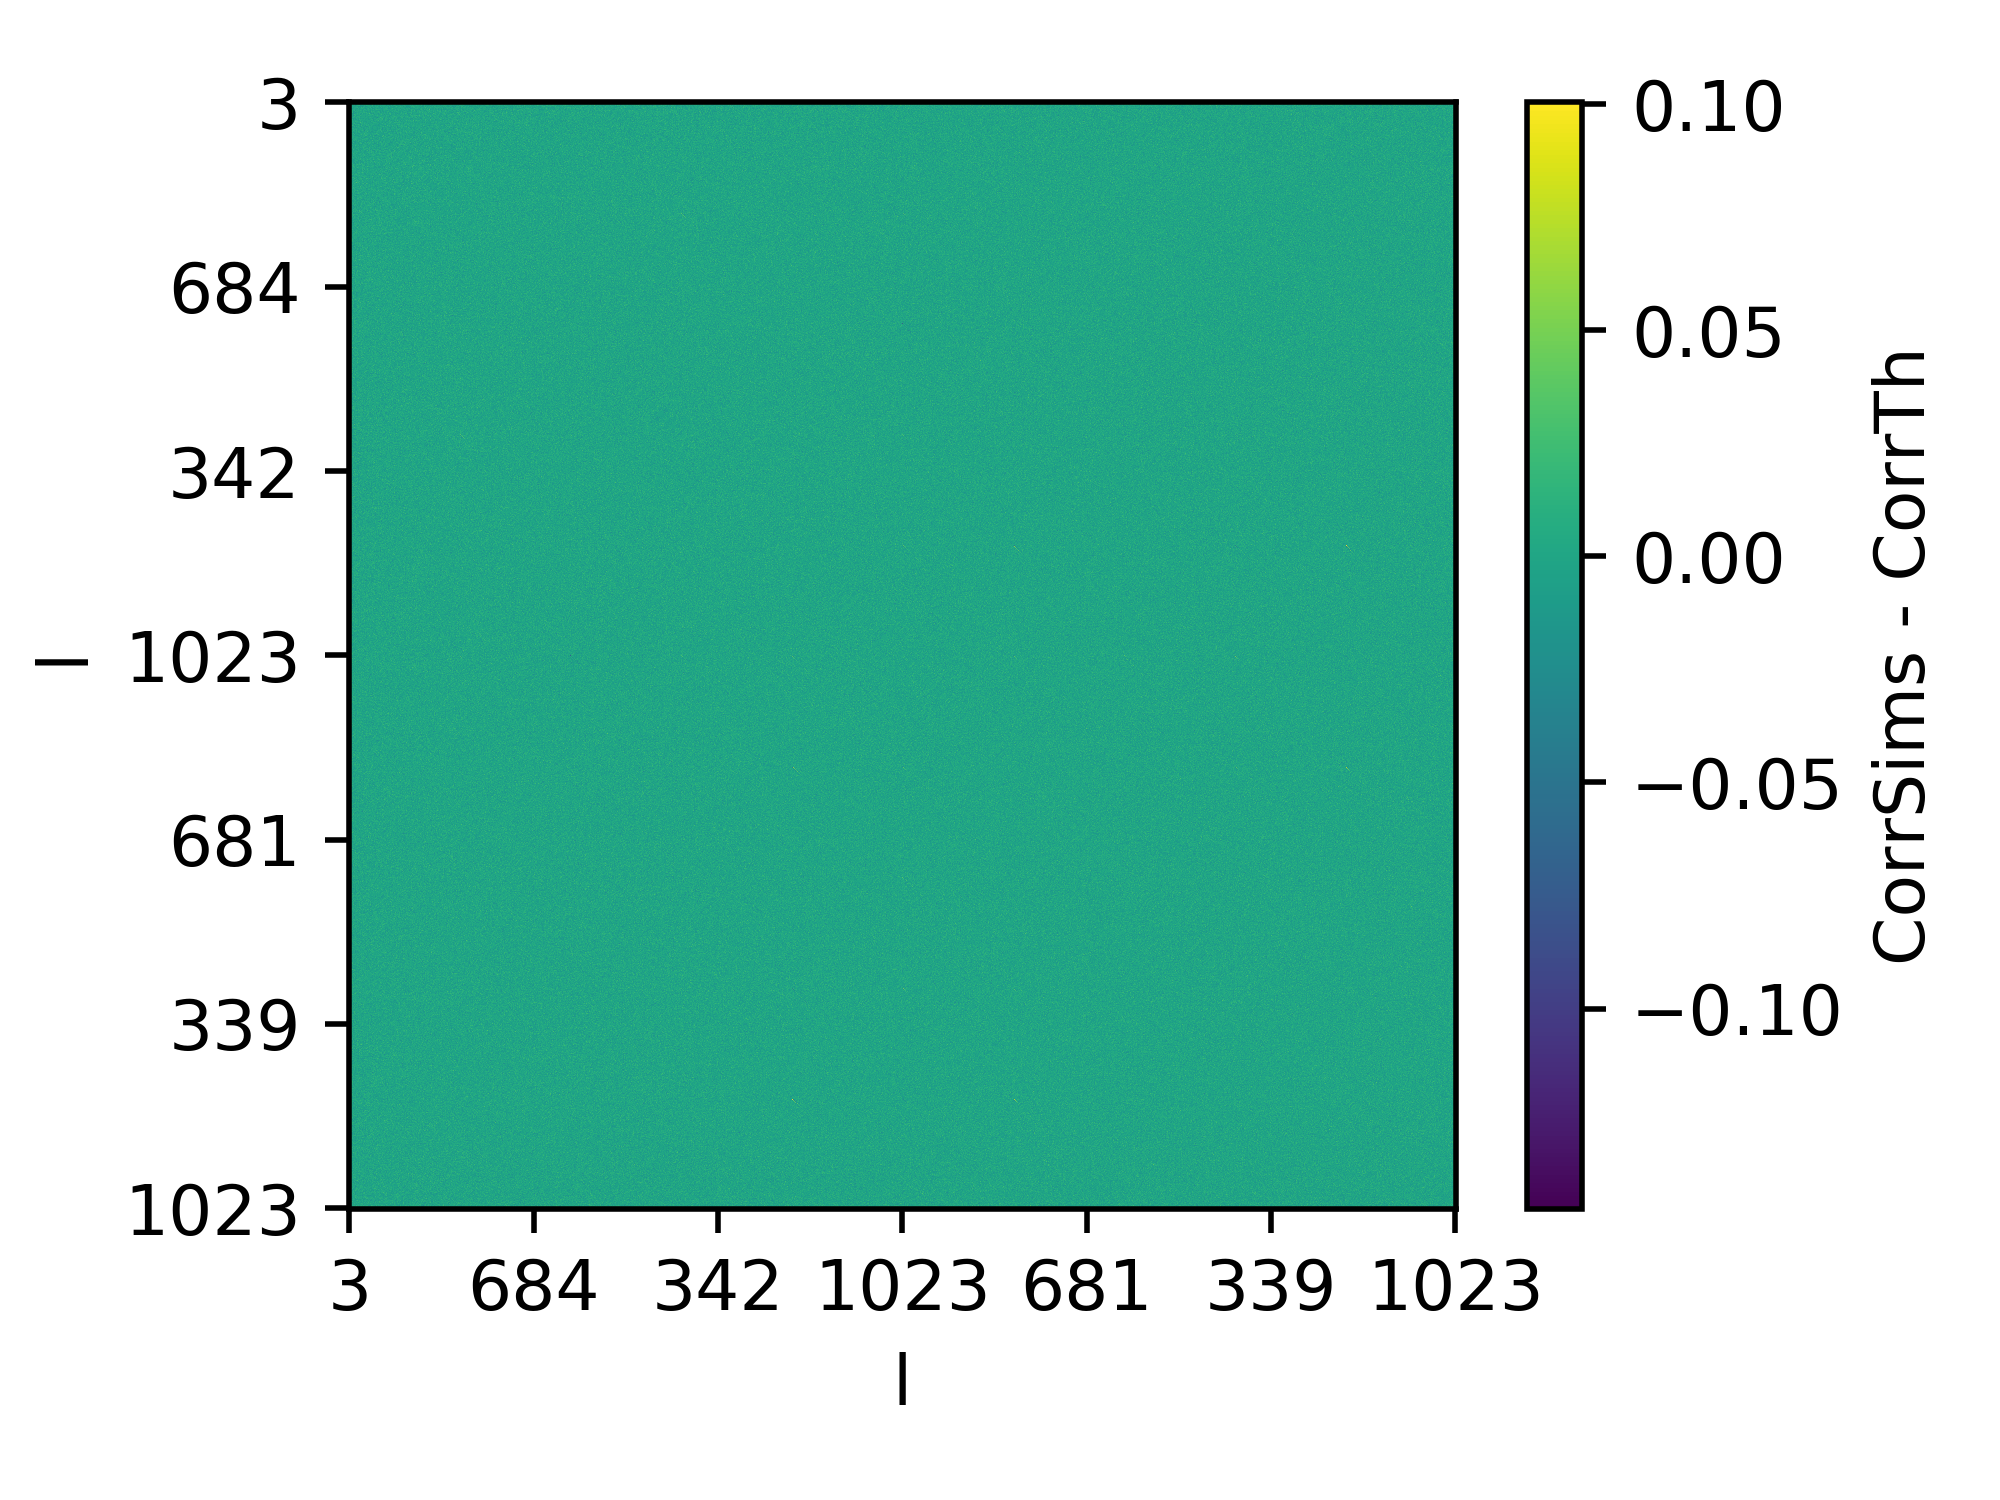
\includegraphics[width=\columnwidth]{./figures/run_sph_2b_same_mask_Efstathiou_TTTEEE_Full_correlation_difference.png}
  \caption{Difference of the correlation matrices of the simulated $\cl$ and
    the analytical one for the modes TT, TE and EE among two bins..}
  \label{fig:TTTEEE_corr}
\end{figure}



% The resulting power spectra was then used to generate a map of the sky and
% two random fields (one of spin-0 and other of spin-2), in turn. Their
% correlations give  are used to obtain the simulated power spectra. In order to
% find the real power spectra, it is necessary to subtract the contribution of
% the mask, which mixes the closest modes:
% \begin{equation}
%   C^{obs}_l = \sum_{l'} M_{ll'} C_{l'}\,
% \end{equation}
% where $M$ depends on the mask. In general, $M$ is not invertible and, in order
% to be able to recover the true power spectra, $C_l$, one needs to bin the
% $l$-space. The bin width is given by the characteristics of the window
% function and must be, approximately, of the size of the range of the mixed
% modes. That way, each $\tilde C_l$ is almost independent of the others
% $\tilde C_{l'}$, and $M$ is invertible.


\section{Discussion}\label{sec:discussion}


\section*{Acknowledgements}
We would like to thank Eva-Maria Mueller for useful discussion. CGG is
supported the Spanish grant BES-2016-077038, partially funded by the ESF and by
AYA2015-67854-P from the Ministry of Industry, Science and Innovation of Spain
and the FEDER funds. He was partially supported by a Balzan Fellowship while
in Oxford. He would like to thank New College and the Department of Physics at
Oxford for their hospitality. DA acknowledges support from STFC through an
Ernest Rutherford Fellowship, grant reference ST/P004474/1.

\appendix

\section{Flat sky}

\setlength{\bibhang}{2.0em}
\setlength\labelwidth{0.0em}
\bibliography{paper.bib}

\end{document}
